\documentclass[oneside,english,master=wtk,inputenc="utf8"]{kulemt}
\setup{title={Path planning algorithm for semi-autonomous mobile robots with fast and accurate collision checking}}
\setup{author={Kevin Denis},
           promotor={Prof.\,dr.\,ir.\ E.~Demeester \and Prof.\,dr.\,ir.\ H.~Bruyninckx},
           assessor={Prof.\,dr.\,ir.\ C.~Tampère \and Dr.\,ir.\ E.~Aertbeliën},
           assistant={Dr.\ J.~Philips}}

% The following \setup may be removed entirely if no filing card is wanted
\begin{comment}
\setup{filingcard,
  translatedtitle=,
  udc=621.3,
  shortabstract={Here comes a very short abstract, containing no more than 500
    words. \LaTeX\ commands can be used here. Blank lines (or the command
    \texttt{\string\pa r}) are not allowed!
    \endgraf }}
\end{comment}
%\setup{coverpageonly} % Uncomment the next line for generating the cover page
%\setup{frontpagesonly} % only the first pages

\setup{font=lm}
%\maxtocdepth{subsection}

% Extra LaTeX packages
\usepackage[numbers]{natbib}
\usepackage{graphicx}
\graphicspath{{./figures/}} % add sub folder figures to LaTeX
\usepackage[T1]{fontenc} % ° in text
\usepackage{amsmath}
\usepackage{amssymb}
\usepackage{textcomp}
\usepackage{units}
\usepackage{nicefrac}
%\usepackage{subfloat} % sub figures 1.a 1.b
%\usepackage{caption}
\usepackage{bm}
\usepackage{tikz-qtree}
\usetikzlibrary{trees}
\usepackage{calc}
\usepackage{subcaption}
\usepackage {optidef} % Constraint Optimisation Problem
\usepackage{mathtools} % align matrixes l m r
\usepackage{gensymb} % \degree in math
\usepackage[chapter]{algorithm}
\usepackage{algorithmicx}
\usepackage[noend]{algpseudocode}
\usepackage{enumitem}
\usepackage{todonotes}
\usepackage{comment}
\usepackage{etoolbox}
\usepackage{titletoc}
\usepackage{stdclsdv}
\usepackage{tocloft}
\usepackage{bigints}
%\usepackage{svg}
% keep this at the end
\usepackage[pdfusetitle,colorlinks,plainpages=false]{hyperref} % commented out for printed versions.. 
\usepackage[noabbrev]{cleveref}

% User made shotcuts en commands
\newcommand{\norm}[1]{\left\lVert #1 \right\rVert} 
\newcommand{\ts}{\textsuperscript}
\setlist[itemize,enumerate]{noitemsep, nolistsep}
\newcommand{\nf}{\nicefrac}

\newcommand*\doublecaption[2]{\caption[#1]{\textsc{#1} #2}}
\algrenewcommand\algorithmicrequire{\textbf{Input:}}
\algrenewcommand\algorithmicensure{\textbf{Output:}}
\algrenewcommand{\algorithmiccomment}[1]{\hfill$\%$ #1}
\algnewcommand{\LeftComment}[1]{\Statex $\%$ #1}

\makeatletter
\patchcmd{\listof}% <cmd>
  {\float@listhead}% <search>
  {\@namedef{l@#1}{\l@figure}\float@listhead}% <replace>
  {}{}% <success><failure>
\makeatother

\renewcommand*\listalgorithmname{}

\makeatletter
\newcommand*\listoffta{%
  \chapter\listofftaname
  \def\@lofmaketitle{\section*\listfigurename}%
  \listoffigures*%
  \let\listoffigures\relax
  \def\@lotmaketitle{\section*\listtablename}%
  \listoftables*%
  \let\listoftables\relax
  \begingroup
  \let\clearpage\relax
  \section*{List of Algorithms}
  \vskip-28.1mm
  \listofalgorithms
  \endgroup}
\newcommand*\listofftaname{List of Figures, Tables and Algorithms}
\makeatother

%\includeonly{chap1-intro}
%\includeonly{chap2-litstudy}
%\includeonly{chap3-design}
%\includeonly{chap4-eval}
%\includeonly{chap6-futwork}
%\includeonly{chap7-concl}

\begin{document}

\begin{preface}
I discovered my passion for autonomous mobile robots during my master thesis in engineering technology (\emph{industrieel ingenieur}), when I had to make an autonomous robot move, starting from an autonomous vacuum cleaner and a few extra sensors for localization and navigation purposes. 
\hbadness=10000 \\ \\
This passion led me to my current studies in engineering science (\emph{burgerlijk ingenieur}). 
The reason for this is twofold. Firstly, I wanted to expand my knowledge of robotics and mechatronics, which are in my eyes the most fascinating domains in engineering today. 
Secondly, I saw it as a personal challenge to do both masters, which is not that common, because of the distinct nature and complementarity of these studies. One is focusing more on the practical side, the other on the conceptual side.
\hbadness=10000 \\ \\
This thesis symbolizes for me the end of my studies, which have become a critical chapter in my life. I would like to thank the following persons who assisted me all along the development of my thesis.  Without their precious help, I would not have been able to write it:
\\
My promoter, Eric Demeester, who presented to me this fascinating thesis topic and who helped me every step of the way during my thesis-journey.
\\
My promoter, Herman Bruyninkxs, for the fruitful discussions and critical eye on the work I produced during this year.
\\
My mentor Johan Philips, who was always available when I needed help.
\\
My supervisors, Chris Tampère and Erwin Aertbeliën, who gave me meaningful advice and input, especially during my midterm presentation.
\hbadness=10000 \\ \\
I would also like to thank my parents, who encouraged me during those intensive years of my student life and who support many of my undertakings.
\hbadness=10000 \\ \\
\emph{Et bien sûr, le meilleur pour la fin ! Merci Alisson, pour ces 6 merveilleuses années passées à tes côtés, pleines d'amour, de tendresse et de soutien. J'ai hâte d'ouvrir ce nouveau chapitre de ma vie avec toi \dots}
\end{preface}

\tableofcontents*

\begin{abstract}
\vspace{-1.03em}
This thesis aims to improve the current local path planning algorithm developed at the Department of Mechanical Engineering of the KU Leuven. The algorithm is used in the context of navigation assistance of electric-powered wheelchairs for the elderly or disabled. The paths obtained from the local path planner are used to model the wheelchair user's intention as well as the path the wheelchair will take. This assistance will help the user to navigate more effectively in challenging situations such as passing through narrow door openings.

Based on the Local Path Template method, which consists of a fixed set of paths starting from the current position and orientation of the robot, the planning algorithm uses an efficient lookup table to adjust each individual trajectory length according to the environment, to obtain collision-free paths.

The current algorithm only uses circular local paths, which is only a small subset of the feasible trajectories a wheelchair can execute. The main contribution of this thesis is to expand this set of local paths by using another curve geometry, the clothoid, a curve whose curvature changes linearly with its arc length. These different paths are generated by using a local version of the State Lattice method, creating Motion Primitives which comply with the wheelchair's kinematic constraints. 

A conceptual solution is presented to enable this new path planner to plan a path considering dynamic obstacles. By using a motion model of a moving obstacle, the dynamic planner calculates a safe velocity profile for the fixed set of paths to yield a collision-free motion along each path.

Other aspects highlighted in this thesis include human-aware robot navigation, a novel research area combining robot navigation with the emerging research area of human-robot interaction. This combination will enable the design of a socially compliant path planner which inherently respects non-written rules of human interaction. A human-robot cooperation model developed in recent literature will be presented as a possible solution to enable the wheelchair to navigate effectively in densely crowded areas.

In comparison to its predecessor the circular path planner, the developed clothoid-based planner achieves substantially improved planning capacity when a more complex path is needed to reach a certain goal. This comes at a cost: the clothoid planner generates six times more paths than the circular planner, which in total take four times longer to process.
\end{abstract}

\begin{abstract*}
\vspace{-1.03em}
Deze thesis heeft tot doel de huidige lokale padplanningsalgoritme ontwikkeld aan het Departement Werktuigkunde van de KU Leuven te verbeteren. Het algoritme wordt gebruikt voor navigatie assistentie van elektrische rolstoelen voor ouderen of mindervaliden. De paden die worden berekend door de lokale padplanner worden gebruikt om de intentie van de rolstoelgebruiker te modelleren, evenals het pad dat de rolstoel zal nemen. Deze assistentie helpt de gebruiker om efficiënter te navigeren in moeilijke situaties, zoals door smalle deuropeningen te gaan.

Op basis van de Lokale-Padsjabloon methode, die bestaat uit een vaste set van paden die afkomstig zijn van de huidige positie en oriëntatie van de robot, gebruikt het padplanningsalgoritme een efficiënte opzoektabel om elke individuele trajectlengte aan de omgeving aan te passen om botsingsvrije trajecten te verkrijgen.

Het huidige algoritme gebruikt enkel circulaire lokale paden, die slechts een klein deel van de trajecten vertegenwoordigen die een rolstoel kan uitvoeren. De belangrijkste bijdrage van deze thesis is het uitbreiden van deze reeks lokale paden door gebruik te maken van een andere curve geometrie, de clothoïde, een kromme waarvan de kromming lineair verandert met zijn booglengte. Deze verschillende paden worden gegenereerd door gebruik te maken van een lokale versie van de State Lattice methode, waardoor bewegingsprimitieven worden gecreëerd die voldoen aan de kinematische beperkingen van de rolstoel.

Deze thesis stelt een conceptuele oplossing voor om de nieuwe padplanner in staat te stellen een pad te plannen dat rekening houdt met dynamische obstakels. Door een bewegingsmodel van een obstakel te gebruiken, berekent de dynamische planner een veilig snelheidsprofiel voor het vaste set van paden om een botsingsvrije beweging langs elk pad te genereren.

Andere aspecten die in deze thesis aan bod komen zijn onder meer mensbewuste robotnavigatie, een nieuw onderzoeksgebied dat robotnavigatie combineert met het opkomende onderzoeksgebied van mens-robot interactie. Deze combinatie zal het ontwerp van een sociaal aanvaardbare padplanner mogelijk maken die ongeschreven regels van menselijke interactie respecteert. Een mens-robot samenwerkingsmodel ontwikkeld in recente literatuur wordt voorgesteld als mogelijke oplossing om de rolstoel effectief te besturen in een dichte menigte.

Vergeleken met zijn voorganger, de circulaire padplanner, levert de clothoïde-gebaseerde planner een aanzienlijk verbeterde planningscapaciteit wanneer een meer complex pad nodig is om een bepaald doel te bereiken. Dit heeft echter een prijs: de clothoïde-planner genereert zes keer meer paden dan de circulaire planner, wat gezamenlijk vier keer langer duurt om te verwerken.
\end{abstract*}

\listoffta

\chapter{List of Abbreviations and Symbols}
\section*{Abbreviations}
\begin{flushleft}
\renewcommand{\arraystretch}{1.1}
\begin{tabularx}{\textwidth}{@{}p{14mm}X@{}}
CEP		& Candidate End Pose \\
COP		& Constrained Optimization Problem \\
DMP		& Discrete Motion Planning \\
DOF		& Degree Of Freedom \\
EP			& Expansion Position \\
FRP		& Freezing Robot Problem \\
ICR			& Instant Center of Rotation \\
LPP		& Local Path Planner \\
LPPA		& Local Path Planning Algorithm \\
LPT		& Local Path Template \\
LSL		& Local State Lattice \\
MP			& Motion Primitive \\
MSG		& Multi-Size Grid \\ 
OG			& Occupancy Grid \\
ROI			& Region Of Interest \\
sAMR		& semi-Autonomous Mobile Robot
\end{tabularx}
\end{flushleft}

\newpage

\section*{Symbols}
\begin{flushleft}
\renewcommand{\arraystretch}{1.1}
\begin{tabularx}{\textwidth}{@{}p{16mm}X@{}}
$v$					& Linear velocity $(\nf{m}{s})$ \\
$\omega$   	& Angular velocity $(\nf{rad}{s})$  \\
$F$					& Force $(N)$ \\
$u_{right,left}$ & Right, left wheel rotational velocity $(\nf{rad}{s})$ \\
$b$ 					& Distance between both driven wheels $(m)$ \\
$r$   				& Turning radius, distance to the instant centre of rotation $(m)$\\
$\kappa$  		& Curvature $(\nf{1}{m})$ \\
$\kappa'$		& Change in cruvate per unit of length $(\nf{1}{m^2})$ \\
$d\theta$		& Angular discretization $(rad)$ \\
$\{R\}$ 			& Local reference frame of the robot \\
$\{I\}$ 				& Inertial or global reference frame \\
$P$ 				& 2D point or position $[x, y]$ \\
${p}$				& Pose $[x,y,\theta]$ \\
$\bm{p_s},\bm{p_0}$ 	& Start pose $[x,y,\theta]$ \\
$\bm{p_e},\bm{p_1}$  	& End pose $[x,y,\theta]$ \\
$\bm{p_{grid}}$ & Candidate End Pose  $[x,y,\theta]$\\
$\bm{P_{grid}}$ & Matrix containing all the Candidate End Poses $[\bm{x},\bm{y},\bm{\theta}]$ \\
$k$					& discrete index \\
$\bm{B}$ 		& Bézier curve $[\bm{x}, \bm{y}]$\\
$u$					& Parameter to construct the Bézier curve $(u =0:\Delta u:1)$ \\
$n$					& Amount of control points of the Bézier curve (order = $n-1$) \\
$L_{tot}$		& Total length of a path ($\bm{s}(end)=L_{tot}$) $(m)$\\
$\mathcal{LSL}$ 	& Local State Lattice data structure\\
$\mathcal{P}$ 		& Path data structure, one entry of $\mathcal{LSL}$  \\
$\mathcal{C}$ 		& Cells of the precomputed lookup table\\
$\bm{XY\Theta}$ 	& Discrete set of poses along a precomputed path \\
$\bm{s}$ 				& Discrete lengths along a precomputed path  \\
$\bm{\kappa}$ 		& Discrete curvature along a precomputed path   \\
$blockIdx$ 				& Last row index of a precomputed path yielding a collision-free path   \\
$pathID$  				& Unique identification number of a precomputed path \\
$pathIdx$ 				&	Row index accessing precomputed data ($\bm{XY\Theta}$, $\bm{s}$, $\bm{\kappa}$)
\end{tabularx}
\end{flushleft}

% Now comes the main text
\mainmatter
\chapter{Introduction} \label{cha:Intro}

\section{Regaining Mobility through Wheelchair Assisted Navigation}
The ability to move around to any desired location is critical to all human activity and interaction. With the increase in average age in Western societies, the loss of mobility caused by reduced physical capacity frequently leads to a loss in social contact and therefore quality of life. Given the scale of this phenomenon, reduced mobility should be addressed as a societal problem and not just as one individual's fate \cite{PrasslerEtAl1999}.

The use of robotic technologies can give back a level of mobility and sense of autonomy to the elderly or disabled. An electric-powered wheelchair enables a person with motion impairment to regain movement control and thus re-engage in more frequent human interactions. However, this renewed mobility brings about its own constraints. Wheelchairs are relatively large compared to their indoor environment (corridors, elevators and other narrow passages). In order to realize the fine maneuvers to navigate the chair without colliding in such environment, a significant degree of dexterity is needed. These tasks are even more demanding due to the non-holonomic characteristics of most wheelchairs. It is therefore often a tiresome and frustrating task for elderly and disabled people to control their wheelchair properly \cite{DemeesterEtAl2003}.

Navigation assistance algorithms have been developed to lower the user's workload for maneuvering their wheelchair. This is done by estimating the navigation intention of the driver and modifying driver's actions if needed to obtain a safer path. The secure implementation of assisted navigation requires, however, the correct interpretation of the user's steering signals and the understanding of the static and dynamic environment \cite{DemeesterEtAl2012a}. In order to obtain effective integrated navigation, shared control over the wheelchair movement is required, building on the respective strengths of the driver (for global planning) and the robotic system (for precise motion control) \cite{DemeesterEtAl2003}. 

An electric wheelchair, equipped with sensors needed to perceive the environment and estimate the user's input signals will also be called a semi-Autonomous Mobile Robot (sAMR) or simply robot in this thesis.

\newpage

\section{Current Research at the Department of Mechanical Engineering} \label{sec:CurrentResearch}
\begin{figure}[!htbp]
\centering
\includegraphics[width=0.75\textwidth]{ElectricWheelchair.jpg}
\doublecaption{Example of a commercially available wheelchair upgraded with Navigation Assistance Technology.}{Added are a custom-made haptic interface, laser scanners perceiving the environment and encoders for a more accurate position measurement (from \cite{DemeesterEtAl2012a}). \label{fig:ElectricWheelchair} }
\end{figure} \noindent
The department of Mechanical Engineering of the KU Leuven has already provided significant contributions to the domain of Wheelchair Navigation Assistance through various projects, including the RADHAR project (Robotic ADaptation to Humans Adapting to Robots) \cite{RADHARWebPage}. The following studies \cite{DemeesterEtAl2012b,DemeesterEtAl2012a,DemeesterEtAl2012,VanderPoortenEtAl2012,VanderPoortenEtAl2012a} are briefly presented to introduce the current status of the research and its challenges. The domain of Wheelchair Navigation Assistance can be divided in 3 main research areas: (i) assessment of the navigation intention of the driver; (ii) generation of a local set of feasible paths to model the driver’s navigation intention; and (iii) haptic feedback for shared control, needed for a better interaction between the driver and the motion controller. These are discussed respectively in \cref{sec:PlanRec,sec:ColFreeTraj,sec:SharedControl}. But first, a brief overview of the robotic platform is given in \cref{sec:WheelchairPlatform}.

\subsection{Wheelchair Platform} \label{sec:WheelchairPlatform}
This section discusses the kinematic model of the wheelchair, the constraints to defining feasible trajectories as well as the mapping of the joystick deflection to an executed motion by the wheelchair.
\subsubsection{Wheelchair Kinematic Model}
The electric-powered wheelchair used at the Department of Mechanical Engineering (shown in \cref{fig:ElectricWheelchair}) is a differentially driven vehicle controlled with a joystick. The rotational speed of the two driven wheels can be controlled separately ($u_{right},u_{left}$). The relation between the linear ($v$) and angular ($\omega$) velocity of the wheelchair and the rotational speed of the wheels is given in \cref{eq:DifferentialDriveModel}. ($v,\omega$) are taken with respect to the local wheelchair coordinates frame ($\{R\}$). The equation on the right relates the linear velocity with the angular velocity and the turning radius ($r$), which is also shown in \cref{fig:DifferentialDriveModel} \cite{VanderPoortenEtAl2012}. 

The non-holonomicity of the wheelchair is expressed in \cref{eq:NonHolonDiffDrive}. The wheelchair can only move (instantaneously) in a straight line (along $x_R$) with respect to the local reference frame ($\{R\}$) and/or turn $(\theta_I)$ with respect to an inertial frame ($\{I\}$). This causes challenging situations for the user when performing maneuvers (e.g. passing through a narrow doorway). In addition to the forward-driven wheels, there are also castor wheels, which are not actuated and rotate freely, adapting the driving direction of the wheelchair. These wheels stabilize the wheelchair, but disturb \cref{eq:DifferentialDriveModel}. Their impact is significant when not orientated in the direction of the wheelchair \cite{VanderPoortenEtAl2012}.

To obtain the position with respect to the fixed inertial frame ($\{I\}$), the linear and angular velocities should be integrated as shown in \cref{eq:InertialReferenceFrame}. A visual representation of this is presented in \cref{fig:InertialReferenceFrame}. 

\begin{figure}[!htbp]
\centering
\includegraphics[width=0.5\textwidth]{InertialReferenceFrame.pdf}
\doublecaption{Position and orientation of the sAMR with respect to the inertial reference frame ($\{I\}$).}{\label{fig:InertialReferenceFrame}}
\end{figure}

\begin{align}
v &= \frac{r_{wheel}(u_{right} + u_{left})}{2} & \omega &= \frac{r_{wheel}(u_{right} - u_{left})}{B} & v &= r \cdot \omega \label{eq:DifferentialDriveModel} \\
\dot{x}_R &= v & \dot{y}_R &= 0 & \dot{\theta}_I &= \omega \label{eq:NonHolonDiffDrive} \\
x_I &= \int v(t) \cdot \cos \theta_I(t) \, dt & y_I &= \int v(t) \cdot \sin \theta_I(t) \, dt & \theta_I &= \int \omega(t) \, dt \label{eq:InertialReferenceFrame}
\end{align}

\begin{figure}[!htbp]
\centering
	\begin{minipage}[b]{.45\linewidth}
		\centering
		
\includegraphics[width=\textwidth]{DifferentialDriveModel.pdf}
	\end{minipage}
	\hfill%
	\centering
	\begin{minipage}[b]{.5\linewidth}
		\centering
		\includegraphics[width=\textwidth]{JoystickWheelchair.pdf}
	\end{minipage}\\[-7pt]
	\begin{minipage}[t]{.45\linewidth}
		\doublecaption{Differential drive model of the wheelchair.}{At each instant, the turning radius $r$ is determined by the rotational velocities of the wheels. If both are equal and in the same direction, the wheelchair will go straight ($ r= \infty $). If both are equal but in opposite direction, the wheelchair will turn on the spot ($r=0$).  \label{fig:DifferentialDriveModel}}
	\end{minipage}
	\hfill
	\begin{minipage}[t]{.5\linewidth}
		\doublecaption{Joystick deflection used to control the wheelchair.}{Each deflection of the joystick ($x_j,y_j$) with respect to the joystick reference frame $\{j\}$ corresponds to a particular circular motion ($v,\omega$) executed by the wheelchair. The slashed-line on the $\{j\}$ frame corresponds to one particular circular path with radius $r$ drawn in dotted lines. The speed and direction is determined by the position $r_j$ (adapted from \cite{VanderPoortenEtAl2012}). \label{fig:JoystickWheelchair} }
	\end{minipage}\\[-14pt]
\end{figure}

\subsubsection{Kinematic Constraints}
In addition to the non-holonomic constraints, further constraints are implemented to obtain paths comfortable to the user. Although a differential drive robot does not suffer from restrictions on the minimum turning radius as a car-like vehicle, a limit on the minimum turning radius ($r$) is implemented. This, to avoid discomfort to the user due to the large centripetal acceleration caused by a small turning radius ($a_c= r^{-1} \cdot v^2$). Based on the guidelines for human-comfortable navigation \cite{MoralesEtAl2013}, a limit on the minimal turning radius ($r \geqslant 1~m$) is introduced (same as in \cite{DemeesterEtAl2003}). Turning on the spot is allowed only if the wheelchair is not in motion.

\subsubsection{Wheelchair Motion Input}
The user can transmit his commands by using a 2 Degree Of Freedom (DOF) joystick shown in \cref{fig:JoystickWheelchair}. The deflection of the joystick $(x_j,y_j$) with respect to the joystick reference frame ($\{j\}$) will directly correspond to a desired linear and angular velocity of the wheelchair as shown in \cref{eq:InputJoinsic}. ($ k_v,k_{\omega}$) are tuneable velocity gains. Each joystick position corresponds therefore to a circular path with radius $r=|v / \omega|$ taking at a speed proportional to $r_j=\sqrt{x^2_j+y^2_j}$. The slashed line in \cref{fig:JoystickWheelchair} corresponds to the dotted circular path taken at different speeds and directions (forwards or backwards) \cite{VanderPoortenEtAl2012}.

\begin{align}
v &= k_v \cdot y_j & \omega &= -k_{\omega} \cdot x_j \label{eq:InputJoinsic}
\end{align}

\subsection{Plan Recognition} \label{sec:PlanRec}
To improve the assistance provided, the navigation intention of the driver is estimated. The intention at time instant $k$ ($\bm{i_k}$) can be expressed as a succession of desired robot states to a goal state $\bm{i_k} = \{\bm{x_{current}}, \cdots,\bm{x_{goal}}\}$. The robot state is defined as $\bm{x} = [x,y,\theta,v,\omega]^T$. 

To generate a set of plans which will serve as a hypothesis for the user intention, possible goal states are connected with feasible trajectories (the latter will be discussed in the next section). Goal states can be known a priori, by asking a user to indicate them on a map or can be generated by recording places where the user stops regularly.

The last step is to assign and update a certain probability ($p$) for each calculated plan as shown in \cref{eq:PathProbUser}. Bayes' theorem is used to compute the posterior probability on $\bm{i_k}$ which is dependent on the user actions sent ($\bm{u}_k$) and a history ($\bm{\mathcal{H}}$) of the user inputs, robot actions, robot poses and sensor readings. $p_{prior}$ is the previous probability distribution on the set of paths and $p_{user}$ is a user model, based on how the user transforms a particular intention into a certain input. This model is calibrated by asking the user to follow a predefined path. $\eta$ is a scale factor normalizing the probability distribution \cite{DemeesterEtAl2012a}.

\begin{equation}
p_{post}(\bm{i}_k | \bm{u}_k, \bm{\mathcal{H}}_{0:k}) = p_{user}( \bm{u}_k | \bm{i}_k , \bm{\mathcal{H}}_{0:k}) \cdot p_{prior}(\bm{i}_k | \bm{\mathcal{H}}_{0:k}) \cdot \eta \label{eq:PathProbUser}
\end{equation}

\subsection{Collision-Free Trajectories} \label{sec:ColFreeTraj}
In order to assess whether a user input signal is collision-free, it is compared to a precomputed set of discrete motions. These motions consists of a set of circular paths defined by ($v,\omega$) pairs. Each precomputed path is associated with a time ($dt$) before a collision occurs while taking this path, which is continuously updated. A path yielding a low $dt$ is considered dangerous and will therefore be subject to a higher correction by the controller \cite{DemeesterEtAl2012}. The way a controller executes this action will be discussed in the next section. \Cref{fig:NavIntSum} shows the collision-free trajectory generation (left) and plan recognition (right).

\begin{figure}[!htbp]
\centering
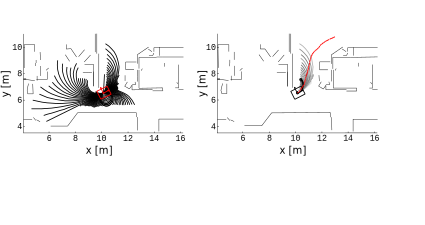
\includegraphics[width=0.8\textwidth]{NavIntSum.pdf}
\doublecaption{Plan recognition based on collision-free trajectories.}{\newline(left) Collision-free trajectories are drawn from the current pose of the robot. (right) Each considered path receives a certain probability (grey-scale, darker color indicates a higher probability). The thick dark precomputed path is locally the best trajectory corresponding to the path (in red) the user will follow (adapted from \cite{DemeesterEtAl2012a}).}
\label{fig:NavIntSum}
\end{figure}

\newpage

\subsection{Shared Control with Haptic Feedback} \label{sec:SharedControl}
When adopting a more traditional scheme of shared control, the user has no direct interaction with the motion controller during the decision-making process. He will only perceive the decided trajectory during the motion of the robot. This can lead to mode confusion \cite{Lankenau2001}, when the path taken by the robot is not the user’s intended plan and even complicates the maneuvering of the wheelchair. This unilateral decision-making scheme is displayed in \cref{fig:SharedControlUni} \cite{VanderPoortenEtAl2012a}. 

To overcome these frustrating situations and to provide a better cooperation between the motion controller and the user, a haptic interface can be used as communication channel. When the current trajectory corresponding to the deflection of the joystick yields a collision in the near future, the haptic interface will provide feedback to the user by ``pushing'' the joystick to a safer direction, while keeping the intention of the user in mind. This interface needs an adapted joystick, featuring additional actuators to provide a certain force ($F_x, F_y$) on the joystick. The user feels at each moment which corrections the controller wants to apply, but is also able to overrule this decision, by applying a higher force as the haptic feedback system, in case a certain direction does not comply with his intention. This bilateral decision-making scheme is displayed in \cref{fig:SharedControlBi} \cite{VanderPoortenEtAl2012a}. 

\begin{figure}[!htbp]
\centering
	\begin{minipage}[b]{.45\linewidth}
		\centering
		\includegraphics[width=\textwidth]{SharedControlUni.pdf}
	\end{minipage}
	\hfill%
	\centering
	\begin{minipage}[b]{.45\linewidth}
		\centering
		\includegraphics[width=\textwidth]{SharedControlBi.pdf}
	\end{minipage}\\[-7pt]
	\begin{minipage}[t]{.45\linewidth}
		\doublecaption{Unilateral decision-making schemes}{don't involve the user in the final decision which can lead to confusion if the selected motion doesn't correspond to the user’s desired motion. Moreover, the user only notices what he perceives as an error in interpretation after the wheelchair has moved (from \cite{VanderPoortenEtAl2012a}). \label{fig:SharedControlUni}}
	\end{minipage}
	\hfill
	\begin{minipage}[t]{.45\linewidth}
		\doublecaption{Bilateral decision-making schemes}{using haptic feedback inform the user of the chosen navigation direction by forcing the joystick to the corresponding position of that motion. If the motion doesn't comply with the user's intention, he can overrule it by forcing the joystick towards his desired position (from \cite{VanderPoortenEtAl2012a}). \label{fig:SharedControlBi}}
	\end{minipage}
\end{figure}

\newpage
\section{Scope and Contribution} \label{sec:contribution}
There is a certain lack of flexibility when only employing circular curves to calculate collision-free trajectories, since circular paths are only a small subset of all feasible motions. When the wheelchair has to pass through a narrow space, from an unfavorable pose as depicted in \cref{fig:EntranceRobotLab} (left) the Local Path Planning Algorithm (LPPA) based on circular arcs only does not find a path going through the doorway. This limits the assistance provided to the user.

This thesis will expand the set of feasible motions by using a more complex curve geometry, thereby offering higher flexibility by being less dependent on the actual pose of the robot as illustrated in \cref{fig:EntranceRobotLab} (right). However, such increased flexibility should be provided while still ensuring fast and accurate collision checking as this has to be performed online. It is therefore important to find a systematic way to create this new set of paths, such that intuitive design parameters can be tuned depending on the complexity of the environment through which the sAMR has to navigate.

\begin{figure}[!htbp]
\centering
	\begin{minipage}[b]{.45\linewidth}
		\centering
		\includegraphics[width=\textwidth]{EnterRobotLabCirc.pdf}
	\end{minipage}
	\hfill%
	\centering
	\begin{minipage}[b]{.45\linewidth}
		\centering
		\includegraphics[width=\textwidth]{EnterRobotLabCloth.pdf}
	\end{minipage}
	\doublecaption{Finding collision-free paths through a narrow doorway depends on the used curve geometry.}{(left) Limited guidance is offered to the user when the collision-free trajectories are only based on circles, as they only represent a limited subset of the feasible paths. (right) Employing curves offering more flexibility will result in feasible paths going through the narrow doorway, thus providing better navigation assistance to the user, less dependent on the current pose of the sAMR. \label{fig:EntranceRobotLab}}
\end{figure}

Two other aspects will also be presented to further improve the LPPA: (i) a conceptual solution to compute the velocity profile for each local path in a dynamic environment given a motion model of the moving objects; (ii) considerations to obtain a socially compliant path planner are developed and the methods needed to enable a planning algorithm in dense crowded environments are shown.

The next section aims to provide an overview of the different aspects that can be considered when designing a Local Path Planner (LPP) and will outline the aspects that will be addressed in this thesis.

\newpage

\section{Requirements for a Local Path Planner} \label{sec:ReqLPP}
%TODO
% Find castor wheels and uncertenties
The task of the LPP is to identify the paths that will be selected in the immediate future. In the context of Wheelchair Navigation Assistance, the LPP also plays the role of providing several feasible trajectories used to model the user's intention. Several additional aspects can be considered to design a reliable LPP in this context. Based on recent literature, these can include: 
\vspace{1em}
\begin{enumerate}
\item Improving user’s intention estimation by widening the range of possible paths \cite{DemeesterEtAl2012,VanderPoortenEtAl2012}.
\item Increase the capacity of the LPP to calculate efficiently more complex paths to assist a wider range of maneuvers in crowded environments including parallel parking and three-point turns for a 180° change in direction \cite{DemeesterEtAl2012,PivtoraikoEtAl2009,ZipsEtAl2016}.
\item Taking into account robot geometry, kinematics and dynamics for path calculations close to the current position of the robot \cite{BouraineEtAl2011,DemeesterEtAl2012,PivtoraikoEtAl2009}.
\item Human-aware path planning, which would greatly improve the effectiveness of navigation in dynamic and crowded environments \cite{KruseEtAl2013,TrautmanEtAl2015}.
\item Accounting for the impact of castor wheels on possible trajectories.
\item Improvements in the way to deal with uncertainties (e.g. in path execution, due to discretisation, etc.) \cite{BouraineEtAl2011,MercyEtAl2016}.
\end{enumerate}
\vspace{1em}

From the above list, this thesis will focus on point 1 and therefore implicitly assist with point 2, when using Discrete Motion Planning (DMP). Point 3 will be partially addressed by providing a conceptual solution for dynamic obstacle avoidance. The paths and collision avoidance will take into account the robot geometry and kinematics. Possible solutions to address point 4 will be presented, to obtain a socially compliant path planner.

\section{Overview} \label{sec:overview}
This thesis is structured as follows: a literature study on path planning algorithms and human-aware navigation is presented in \cref{cha:LitStudy}, providing a review of several methods to generate a set of flexible trajectories and of guidelines to obtain a more socially compliant navigation. The design of a novel LPPA is detailed in \cref{cha:Design} followed by an evaluation of that design in \cref{cha:Eval}. Future work as well as a conclusion of this thesis can respectively be found in \cref{cha:FutWork,cha:Concl}.

There are also two appendices, \cref{app:BezierCurve} further elaborates mathematical concepts of the Bézier curve, one of the considered curves for motion planning. Finally, the content of the source code of the GitLab repository \cite{Denis2017} containing the same information as the digital appendix, is presented in \cref{app:SourceCode}
\chapter{Literature Study} \label{cha:LitStudy}

\section{Introduction}
This chapter presents the literature study performed for this thesis. It consists of two parts: (i) the different path planning algorithms, on which the design of the Local Path Planner (LPP) discussed in \cref{cha:Design} is based and (ii) human-aware robot navigation, a new field in robotics that has received increasing attention from the moment that robots started working in proximity to humans. The latter part will enable the LPP to adopt a more socially compliant navigation.

\section{Path Planning Algorithms}
\Cref{sec:LPTreview} will further review the method to generate collision-free trajectories discussed in \cref{sec:ColFreeTraj} based on the following research \cite{DemeesterEtAl2012}. One of the contributions of the present thesis is to provide a more flexible set of paths, compared to those described in \cite{DemeesterEtAl2012}. Two possible approaches enabling the robot to plan a path through a challenging environment will be evaluated in \cref{sec:SLreview,sec:OMGreview} treating respectively the State Lattice path planning and an Optimal Motion Generation method. Important evaluation criteria are the local nature of the path planner, the scalability with large numbers of obstacles and the ability to provide a set of collision-free paths, which will be used to model the intention of the user.

\subsection{Local Path Template} \label{sec:LPTreview}
The LPP developed by Demeester et al. \cite{DemeesterEtAl2012} is based on the Local Path Template (LPT) method. This LPT consists of a fixed set (or template) of feasible trajectories starting from the robot's current pose (therefore local). A feasible path means that this path respects the robot's kinematic constraints.

Using a fixed set of motions brings several advantages, as the position and orientation of the robot along each path can be calculated in advance (offline) and stored in a lookup table. This lookup table contains which space the robot will take when following a particular path. The online phase consists of efficiently adjusting each path length to obtain collision-free trajectories, by using this precomputed lookup table.

However, the main disadvantage of this LPT comes with the restriction in the number and geometry of the used paths, since it is not efficient to include the full set of feasible paths that can be performed by the robot. A limit on the set must be made, thereby yielding only a (small) subset of feasible paths. However, if there are too many limitations on this set of paths, the robot will be unable to plan an otherwise kinematically feasible path which is not in the LPT. \Cref{fig:EntranceRobotLab} illustrated this problem.

The method used to create kinematically feasible paths in \cite{DemeesterEtAl2012} is to integrate achievable velocities of the wheelchair. This is commonly referred to as the forward generation method. The set of paths is obtained by integrating (maximum) allowable linear and angular velocity ($v$, $\omega$) pairs, over a certain amount of time $\Delta t$, as shown in \cref{fig:MPCircVWPair} (left). This results in a circular LPT in \cref{fig:MPCircVWPair} (right).

The main contribution of \cite{DemeesterEtAl2012} is the method used to adjust each path to obtain collision-free trajectories. This started with the observation that when paths are individually checked for collision, grid cells occupied by the robot at the start of each path are common for the majority of the paths (because all paths start from the current pose of the robot). Individual path-checking therefore results in checking several times the same grid cells, which is not efficient. Instead of building the lookup table based on each path, it can be build based on the cells occupied by the robot. In this case, cells occupied by the robot when taking each path of the LPT contain (i) which path the robot took to occupy this particular cell and (ii) its corresponding path length. The online phase will then consist of matching the occupied grid cells in the environment with cells from the lookup table. If this results in a shorter path length, then the path will be adjusted accordingly. 
\begin{figure}[!htbp]
	\centering
	\includegraphics[width=\textwidth]{MPCircVWPair.pdf}
	\doublecaption{(right) Kinematically feasible motions obtained by integrating achievable robot velocities (left)}{over a period $\Delta t = 4 s$. This results in a circular LPT, composed of 200 circular paths, including forward, backward and on the spot turning (adapted from \cite{DemeesterEtAl2012}).
	\label{fig:MPCircVWPair}}
\end{figure}

\subsection{Sate Lattice} \label{sec:SLreview}
As pointed out in \cref{sec:contribution}, a LPT exclusively based on circular curves will not always find a path in narrow passages when departing from certain start poses. A possible method of building a more flexible set of paths can be found in the research of Pivtoraiko and Kelly \cite{PivtoraikoKelly2005,PivtoraikoEtAl2009,PivtoraikoKelly2012}.

This research introduces a novel search space, the State Lattice, which represents a discrete set of states connected with feasible paths. This set of paths is called Motion Primitives (MPs) and connects nearby grids with trajectories compliant to the robot's motion constraints. \Cref{fig:SL_PP} (left) displays a possible set of MPs, which is then uniformly distributed over the whole grid to obtain the State Lattice search space, shown in \cref{fig:SL_PP} (right).

This method brings with it several advantages. Although the environment is discretized, the path connecting one state to another respects the continuity constraints of the vehicle (in the case of the wheelchair, the non-holonomic constraints). This transforms the ordinary constrained search into a minimization function, since all the connections are feasible. A certain cost should be assigned to each path of the State Lattice, for example proportional to its length, comfort, distance to obstacles.

The main focus of this research is the Global Path Planning Problem. Although this is not directly related to the local path planning, the methods described generating the set of MPs can be used to design a LPP. Pivtoraiko and Kelly describe a systematic method of generating a near-minimal set representing the MPs \cite{PivtoraikoKelly2005}. This method is based on the inverse generation method and consists of the following steps: 
\vspace{1em}
\begin{enumerate}
\item A curve geometry is chosen. For example, a polynomial curve.
\item The geometric state describing the robot are chosen (e.g. $[x,y,\theta]$) and the environment is sampled.
\item Each sampled state in the surroundings of the robot is connected using the chosen curve geometry. This is a constrained boundary value problem as only feasible paths are allowed.
\item In order to obtain a near-minimal spawning set from the origin, the notion of path decomposition has to be introduced. Each path that can be subdivided into previously calculated paths should be discarded. By doing so, an efficient set of paths is obtained resulting in faster searches.
\end{enumerate}

\begin{figure}[!tbp]
\centering
 \begin{minipage}[b]{.45\linewidth}
		\centering
		\includegraphics[width=0.85\textwidth]{SL_MP.jpg}
 \end{minipage}
 \hfill%
 \centering
 \begin{minipage}[b]{.45\linewidth}
	\centering
	 \includegraphics[width=0.85\textwidth]{SL_PP.jpg}
 \end{minipage}\\[-7pt]
 \begin{minipage}[t]{.45\linewidth}
 \end{minipage}
 \hfill
 \begin{minipage}[t]{.45\linewidth}
 \end{minipage}
	 \doublecaption{State Lattice search space based on a set of feasible motions.}{(left) A set of MPs is obtained by connecting end poses (states) with feasible trajectories from the origin. (right) By repeating the MPs uniformly, an efficient search space is obtained called the State Lattice, consisting only of feasible connections between states. An optimal path between a start- and end pose is found by minimizing an objective function represented by the cost to travel from one state to another (adapted from \cite{PivtoraikoEtAl2009}).\label{fig:SL_PP}}
\end{figure}

\newpage

\subsection{Optimal Motion Generation} \label{sec:OMGreview}
The MECO (Motion Estimation, Control and Optimization) research group of the Department of Mechanical Engineering of the KU Leuven has developed a freely available toolbox \cite{MercyVanParys2017} for Optimal Motion Generation. Based on the following research \cite{MercyEtAl2016}, \cite{VanParysPipeleers2016}, \cite{VanParysPipeleers2017}, this toolbox uses spline based motion planning for path planning in an environment including both static and dynamic obstacles. 

Three main challenges arise when trying to find an optimal (in terms of speed, safety and energy consumption) trajectory between a start and end position while respecting the system's constraints and avoiding obstacles \cite{MercyEtAl2016}.
(i) The geometric constraints, obstacle avoidance, kinematic constraints and actuator limits translate into hard non-convex problems. Optimal solutions are not guaranteed because of the local minima and are difficult to find, certainly in real-time. 
(ii) The constraints mentioned in (i) should be respected during the whole motion, not only at discrete time intervals. 
(iii) The environment in which the system operates has a degree of uncertainty. The obtained motion trajectory should be continuously updated using the most recent information on that environment.

These three challenges are addressed by using B-spline parameterization, which guarantees that the constraints are respected at all times \cite{VanLoockEtAl2015}. Time-varying separating hyperplanes are used to enforce collision-free paths along the trajectory as shown in \cref{fig:SeparatingHyperPlane}. This is calculated in real-time and continuously updated to cope with the uncertainty in the perceived environment. A robust path planning tool is obtained by using an appropriate motion model for the obstacles and by updating the planned motion to cope with unknown obstacles. Several scenarios are provided in \cref{fig:OMG_Example} as illustration.

\begin{figure}[!htbp]
	\centering
	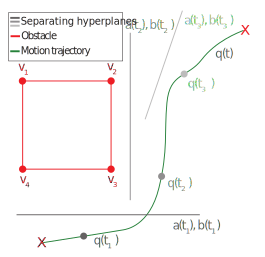
\includegraphics[width=0.5\textwidth]{SeparatingHyperPlane.pdf}
	\doublecaption{Obstacle avoidance obtained by using time-varying separating hyperplanes.}{At each discrete time instant, a hyperplane (a straight line in this 2D example) should be drawn to separate the obstacle from the robot. $a(t)$ and $b(t)$ are the 2 parameters needed to define the hyperplane. $q(t) = [x(t), y(t)]^T$ represents the state of the robot and therefore the motion trajectory to be followed (from \cite{MercyEtAl2016}).\label{fig:SeparatingHyperPlane}}
\end{figure}

\begin{figure}[!htbp]
	\centering
	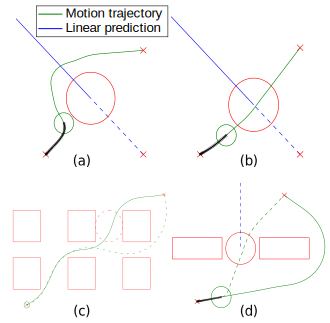
\includegraphics[width=0.59\textwidth]{OMG_Example.pdf}
	\doublecaption{Different examples for Optimal Motion Generation.}{In (a), an inappropriate motion model is assigned to the moving circle (object is assumed static even though it is moving along the blue line), leading to a possible collision. (b) Uses a correct obstacle motion model yielding a safe trajectory. In (c) an unexpected additional obstacle (dashed lines) is encountered, requiring a different path to the destination to be calculated. In (d), the circular obstacle starts moving, enabling the planner to find a shorter path through the narrow doorway (from \cite{MercyEtAl2016}). \label{fig:OMG_Example}}
\end{figure}

Although this method appears promising to obtain a flexible path, some important problems remain if it were implemented with the current Wheelchair Navigation Assistance scheme, as reviewed in \cref{sec:CurrentResearch}.
\vspace{1em}
\begin{itemize}
\item The current algorithm used to estimate the wheelchair driver's intention needs a whole set of feasible paths, which will result in solving $n$ times a slightly different constrained optimization function. This will result in a slow calculation of the set of feasible trajectories, which is not acceptable in this situation.
\item It is not clear whether (i) this method scales well in a real-world environment with a lot of obstacles and (ii) how the method would cope with non-convex obstacles and robot geometry.
\item By continuously solving a constrained optimization online, the main advantage of having a fixed set of local paths is lost. 
\end{itemize}
\vspace{1em}

The toolbox developed by MECO is particularly well suited for the use in autonomous systems. The method is, however, less adapted to situations where the intention of the user is unknown and must be continuously estimated (like a sAMR). The current intention estimation method needs a whole set of trajectories to work and therefore requires solving several times an optimization function, which necessitates too much time.

\newpage

\section{Human-Aware Robot Navigation}
This section discusses human-aware robot navigation. \Cref{sec:HARNrev} is mostly based on the survey by Kruse et al. \cite{KruseEtAl2013} and articles reviewed as part of their survey. \Cref{sec:HRCrev} focuses on a novel solution based on human-robot cooperation, to solve the ``Freezing Robot Problem'' (FRP), which happens when the robot's surroundings exceed a level of dynamic complexity. This research has been performed by Trautman et al. \cite{TrautmanEtAl2015}, which is the first publication providing a large empirical study to validate their study on navigation techniques in populated environments. This topic is especially relevant for wheelchair navigation in dense human crowds, as solving the FRP will contribute towards safer and more efficient navigation.

\subsection{Rationale and Research Areas} \label{sec:HARNrev}
Path planning for autonomous robots has become a mature field in robotics. Even in environments outside factories or other controlled areas, autonomous systems have proven their robustness in navigation among humans. For example, the research performed by Prassler et al. \cite{PrasslerEtAl1999} in 1999 introduced an autonomous wheelchair navigating in a railway station during rush hour, without any reported collision with pedestrians.

Although not colliding with the environment is an essential skill of any autonomous system, this is certainly not the only important aspect to obtain systems which are accepted and work well alongside humans. A new field focusing on increased awareness by robots of humans in the environment has emerged over the last few years. Human-aware robot navigation combines the field of human-robot interaction and robot motion planning to obtain a robotic system that is not only reliable but also accepted by humans in their new work environments. Whilst this human-robot interaction was not discussed in \cite{PrasslerEtAl1999} as per above, one can only imagine that the obstacle avoidance of the wheelchair consisted of fast and unpredictable evasive maneuvers, or just standing still if no collision-free path was found, both of which can cause confusion for the surrounding crowd. This is not a desirable interaction, as this way of navigating does not take into account that the surrounding crowd can react to and even cooperate with the wheelchair.

According to the research of Kruse et al \cite{KruseEtAl2013}, human-aware robot navigation can be divided in three different fields of research: comfort, naturalness and sociability.

\textbf{Comfort: }
The robot should not cause any stress or annoyance to the humans interacting with it. It should therefore not only be safe but be understood as safe by the interacting humans. The study of proxemics is therefore essential to avoid discomfort. Hall \cite{Hall1966} has conducted an elaborate research on the different comfort zones around a standing person during human-human interaction. Each of the zones are reserved for a different social interaction defined by a distance to the person (intimate, personal, social and public distance). Although these different comfort zones are also used as guidelines for human-robot interaction, it is important to note that the influence of dynamics (moving persons or robots) on these zones has not been properly studied so far. These dynamic factors include among others whether the person is sitting or standing and the shape and size of the approaching robot.

\textbf{Naturalness: }
The robot's behavior on a ``low level'' should reflect human motion patterns. A first step is to mimic human mobility by obtaining a jerkless motion, since humans try to be as energy efficient as possible in their movements \cite{ArechavaletaEtAl2008}. Also, a robot action should be legible (readable), meaning that the interacting humans can interpret the robot's behavior and judge its current and future actions. When a robot has legible actions, it becomes possible to have some form of cooperation between the robot and the human to facilitate the completion of each one's individual task. This is particularly important when planning a motion in a crowded environment. If the robot doesn't anticipate human cooperation, it will be unable to plan a path through or following the crowd and will try to evade it.

\textbf{Sociability: }
The robot's behavior on a ``high level'' should be similar to that of a human. This includes cultural conventions (e.g. lane side right/left) and other social protocols. E.g. skipping people in a lane and going back into the lane could be done without discomforting humans and come across as natural, but is certainly not an acceptable social behavior. Social behavior can also help in the navigation in a crowded environment, since this can be used to predict in some way the motion of pedestrians, which typically form virtual lanes when walking in close formation \cite{Helbing1991}.

\subsection{Human-Robot Cooperation} \label{sec:HRCrev}
From the moment dynamic objects (e.g. humans) in the immediate surroundings of the robot perform movements that are too complex for the path planner; the latter is unable to make suitable decisions and the robot suddenly stops or performs dangerous or unpredictable evasive maneuvers. This phenomenon is commonly referred to as the FRP. As can be seen in \cref{fig:FRP} (left), the robot (black star) tries to predict the future location of the surrounding agents (humans, red ellipses). As there is no precise motion model of the agent's movements, the uncertainty of the agent's location becomes too large for the robot to make an informed decision. It is unable to plan a path to the goal (green star).

A naive solution would be to try to achieve a good individual motion model prediction for the agents. This would work, if the crowd is sparse (\cref{fig:FRP}, right). However, from the moment the crowd is more numerous or adopts a complex formation (e.g. shoulder to shoulder walking) each independent navigation planner is bound to fail as shown in \cref{fig:HuRoCo}. Even if the predictive motion covariance is extremely low, the robot will try to pass around this formation.

\begin{figure}[!htbp]
	\centering
	\includegraphics[width=0.49\textwidth]{FRP1.jpg}
	\hfill
	\includegraphics[width=0.49\textwidth]{FRP2.jpg}
	\doublecaption{The FRP}{(left) is caused by an uncertainty explosion of the agents future location (red ellipses) due to an inaccurate motion model. The robot (black star) is therefore unable to make a decision on how to navigate through this crowd to reach the goal (green star) and stops moving. (right) When having a very low covariance on the motion prediction of each individual agent, the robot is able to plan a path when the crowd is sparse enough (from \cite{TrautmanEtAl2015}).\label{fig:FRP}}
\end{figure}

The authors of \cite{TrautmanEtAl2015} found a possible solution by inspiring themselves on how humans themselves manage to navigate in large dense crowds. Humans typically solve this problem by forming a ``joint collision avoidance'' scheme, where every agent adapts his path according to the surroundings to allow passage for everyone. Therefore, the authors redefined the ill-formulated independent path planner to explicitly expect cooperation from humans. Their method, named Interactive Gaussian Process, models the robot as part of the human crowd, and expects that all agents adapt their path so that everyone can reach their destination.

\begin{figure}[!htbp]
	\centering
	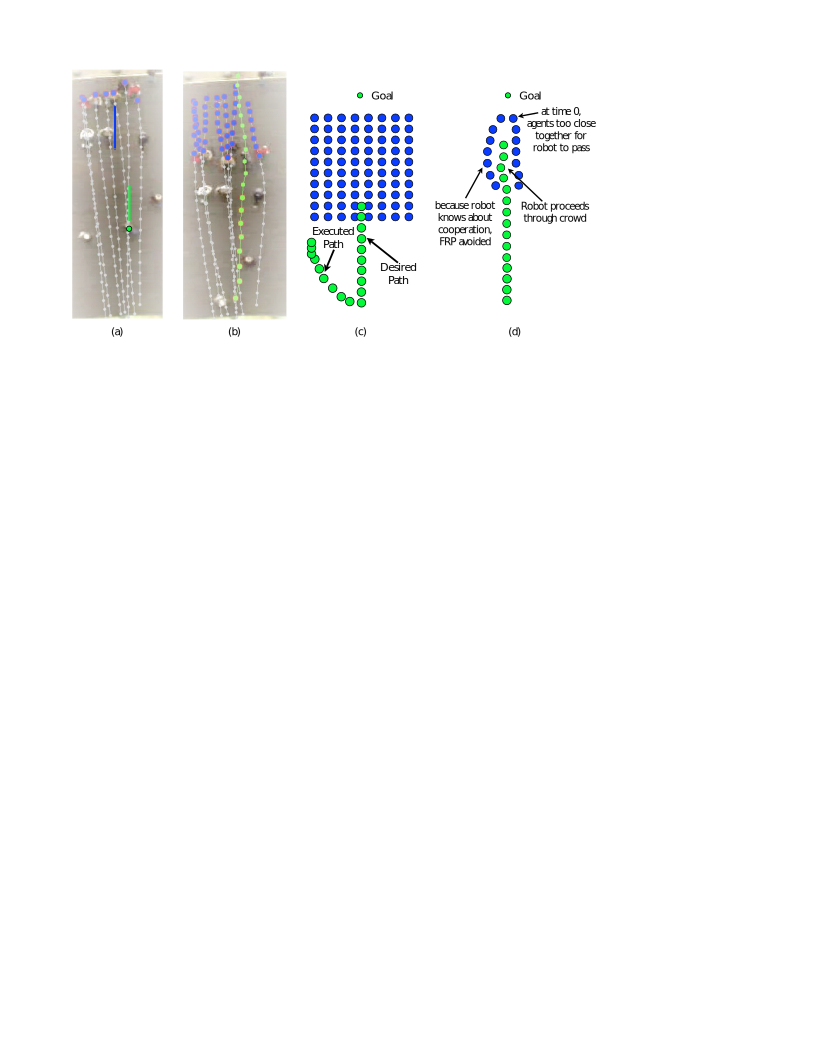
\includegraphics[width=1\textwidth]{HuRoCo.png}
	\doublecaption{Shoulder to shoulder formation makes the robot unable to plan an efficient path when relying on an independent planner.}{(a)-(b) Shows an example of joint collision avoidance. In (a), the group of people (blue dots) has not yet seen the person going up (green dot), their trajectory projection (grey line) is very narrow. In (b), everyone has adjusted their trajectory to create space. (c) Even with perfect motion prediction, the independent motion planner will not capture the cooperation between the robot (green) and the people (blue) and therefore perform an evasive maneuver even though the group of pedestrians is willing to make passage for the incoming robot. (d) Modelling this cooperation avoids the FRP (adapted from \cite{TrautmanEtAl2015}).\label{fig:HuRoCo}}
\end{figure}

\section{Conclusion} \label{sec:ConclusionReview}
The LPP to be designed in \cref{cha:Design} will contribute to the work described in \cref{sec:LPTreview} by using methods elaborated by Pivtoraiko and Kelly (\cref{sec:SLreview}). Important aspects of human-aware navigation will be considered, to obtain a LPP which inherently takes into account important aspects (comfort, naturalness and sociability) of navigation among humans. The integration of the human-robot cooperation model elaborated in \cite{TrautmanEtAl2015} in the LPP is also critical as this will enable to achieve a more robust navigation scheme when navigating in dense crowds and will therefore solve the FRP typically occurring in this type of environment. Whilst mathematical models of this cooperation model are further elaborated in \cref{sec:Cooperation}, they have not been formally implemented within the framework of this current thesis.
\chapter{Design of a Local Path Planner} \label{cha:Design}
\vspace{-1.56em}
\section{Introduction}
The designed LPPA aims to improve the work developed in the Department of Mechanical Engineering of the KU Leuven \cite{DemeesterEtAl2012}, which has been discussed in \cref{sec:ColFreeTraj,sec:LPTreview}. A LPT is used in order to plan a motion, consisting of a fixed set of feasible trajectories starting from the robot's current pose.

The main improvement of the new LPPA is to overcome a shortcoming of the LPT from \cite{DemeesterEtAl2012}, namely the difficulty to plan feasible paths in narrow openings starting from certain poses, due to the lack of flexibility of the applied curve geometry. As only circular curves are used as a basis for the trajectories planned by this LPT, it will be referred to as the circular LPT throughout the rest of this thesis.

The solution employed to address this issue is inspired by the work of Pivtoraiko and Kelly \cite{PivtoraikoKelly2005,PivtoraikoEtAl2009,PivtoraikoKelly2012}, that has been reviewed in \cref{sec:SLreview}. Their methods describe how to generate a set of MPs in order to connect one state (robot pose) to another. The level of complexity of the trajectories depends upon the choice of the curve geometry, the basis of the MP, which will be an important design parameter.

The new LPT is created by using a Local State Lattice (LSL) (a local version of the State Lattice of Pivtoraiko and Kelly) and an obstacle-based lookup table for collision checking to obtain rapidly a set of collision-free paths. Since clothoids will ultimately be chosen as the basis of the MPs, the new LPT as developed in this thesis will be called clothoidal LPT.

The method applied can be summarized in the following steps:
\begin{enumerate}
\item Generation of a multi-size grid (fine close to the robot and coarse far from it).
\item Each grid cell in the Region Of Interest (ROI) around the origin is connected with a geometrical curve. If this path is feasible, it is added to the set of MPs.
\item To ensure a certain degree of flexibility, step 2 is repeated at certain grid cells, called Expansion Positions (EPs). By doing this, certain paths in the LSL will consist of two subsequent curves.
\item The Occupancy Grid (OG) is calculated for each path, by using the geometry of the wheelchair. A lookup table is built for this fixed set of trajectories to quickly assess if a motion is collision-free and where the collision occurs.
\item The LPPA updates each path by adjusting its length in order to be collision-free within the perceived environment.
\end{enumerate}

Steps 1 to 4 are executed offline. Step 5 is performed in real-time. The collision-free paths calculated by the LPPA are used to model the navigation intention of the wheelchair driver as explained in \cref{sec:PlanRec}. Each path receives a certain probability, reflecting its likeliness to be the true user's intention.

This chapter is structured as follows: first, the construction of the LSL is explained in \cref{sec:LSL}. Then the lookup table for collision checking with a short example of the online phase is presented in \cref{sec:LTCC}. A conceptual solution to extend the LPPA with the ability to plan a motion in a dynamic environment is presented in \cref{sec:DynPlan}. Considerations on socially compliant  path planning are provided in \cref{sec:HAPP}. Finally, a conclusion is given in \cref{sec:DesignConclusion}.

\section{Local State Lattice} \label{sec:LSL}
This section is the first step of the construction of the new LPT, the calculation of the LSL. The LSL constitutes a fixed set of feasible trajectories originating from the robot's current pose. First, the surrounding end poses are discretized (\cref{sec:MultiGrid}). Then a geometric curve is used as basis for the MP in order to connect the origin with achievable end poses (states) (\cref{sec:MPG}). Finally, EPs are added to create a greater variety of paths (\cref{sec:EP}).

\subsection{Multi-size grid and Region of Interest} \label{sec:MultiGrid}
The first step in the creation of the LSL is sampling the reachable space surrounding the sAMR by using a multi-size grid (MSG). This grid is the representation of the discrete poses (states) that the robot will try to reach from his current pose (the origin, in the local reference frame of the robot). The MSG is composed of three different sizes, fine, medium and coarse, as shown in \cref{fig:MultiGirdWithROI}.

This method is the inverse generation method to create a set of MPs. First, the environment is sampled and a boundary value problem is solved to connect these discrete states with feasible paths using a defined curve geometry. The forward approach, which has been used in \cite{DemeesterEtAl2012}, consists in integrating feasible robot velocities, resulting automatically in kinematically feasible paths. The inverse approach is preferred in this implementation as it makes the state discretization the driver of the design of the LSL. Parameters can then be fine-tuned depending on the application.

The main reason to adopt a MSG is to limit the number of paths far away from the origin. It would be inefficient to keep a larger number of paths leading to a pose that is relatively similar with respect to the origin, since the environment and the intention of the driver may change. An end pose located in the coarse grid represents therefore a large group of poses compared to an end pose in the fine grid.

A ROI selects the Candidate End Poses (CEPs) of the grid cells in the immediate surrounding of the origin. This step is illustrated in \cref{fig:MultiGirdWithROI}. Depending on the chosen geometry of the MP and the constraints of the robot, a CEP will be reachable or not. If it is reachable, the path leading to the CEP will be added to the set of MPs. Values of the used parameters and a short description can be found in \cref{tab:LSLParVal}. This table also contains parameters which will be discussed in \cref{sec:LTCC}.

\begin{figure}[!htbp]
\centering
\includegraphics[width=0.90\textwidth]{MultiGirdWithROI.pdf} 
	\doublecaption{MSG and ROI shown at the origin.}{Three different grid sizes are used to sample the environment. Grid cells in the ROI become CEPs, which will be connected to the origin by a geometrical curve. Parameter values are shown in \cref{tab:LSLParVal}. Only feasible trajectories will be added to the set of MPs.\label{fig:MultiGirdWithROI}}
\end{figure}

\begin{table}[!htbp]
\centering
\doublecaption{LSL parameters and corresponding values.}{\label{tab:LSLParVal}}
\vspace{0.2cm}
\begin{tabular}{ r | l | l}
parameter							& 		value			& description	\\ \hline \hline
$dx_1,dy_1$ 						& 		0.10 m 		& Discretization of the fine grid.	\\ \hline
$x_{1,max},y_{1,max}$ 	& 		1.00 m		& Width and height of the fine grid.	\\ \hline
$dx_2,dy_2$ 						& 		0.25 m 		& Discretization of the medium grid.	\\ \hline
$x_{2,max},y_{2,max}$		&		2.00 m		& Width and heigh of the medium grid. \\ \hline
$dx_3,dy_3$ 						& 		0.50 m 		& Discretization of the coarse grid.	\\ \hline
$x_{3,max}$ 						& 		4.00 m		& Width of the coarse grid.	\\ \hline
$y_{3,max}$ 						& 		3.00 m		& Height of the coarse grid.	\\ \hline
$d\theta$							& 		$\pi$/8 rad	& Angular discretization, constant over the whole grid	\\ \hline
$x_{ROI}$ 							&		2.00 m 		& x-distance (only +) defining the ROI.	\\ \hline
$y_{ROI}$							& 		1.50 m		& y-distance (+/-) defining the ROI. 		\\ \hline
$\kappa_{max}$ 				& 		1 m$ ^{-1}$	& Maximum allowed curvature.		 \\ \hline 	
$dx_{EP}$							&		0.50 m		& Manhattan Distance ($\bm{\ell_1}$-norm) between EPs \\ \hline
$res_{OG}$						&		2 cm			& Resolution of the OG\\ \hline 
$res_{path}$						&		1 cm			& Resolution of the path
\end{tabular}
\end{table}
\newpage

\subsection{Motion Primitives Geometry} \label{sec:MPG}
Once the CEPs around the origin are determined, a geometrical connection has to be established between the two robot states. Two possible curve formulations are discussed below, Bézier curves and clothoids. Both have interesting properties to become the basis for the MPs. At the end of this section, the selection of the clothoid will be advocated.

\subsubsection{Bézier curve}
The general form of a Bézier curve of order $n-1$ is shown in \cref{eq:BezierCurveGeneral}. The basis of this curve consists of the Bernstein polynomials, which is the multiplication of the binomial and polynomial coefficients. This is then multiplied by a certain weight, corresponding to the $i^{th}$ control point $P_i$. $n$ represents the amount of control points used to define the Bézier curve \cite{Sederberg2016}.

\begin{equation} \label{eq:BezierCurveGeneral}
\bm{B}(n,u) = \sum_{i=0}^{n-1}
\underbrace{ \begin{pmatrix} n-1 \\ i \end{pmatrix}}_\text{binomial term} \cdot~
\underbrace{(1-u)^{n-1-i} \cdot u^i}_\text{polynomial term}
\cdot~\underbrace{ P_i}_\text{control point}
\end{equation}
Bézier curves are commonly used in Computer Aided Geometric Design Software and are also used in path planning algorithms for mobile robots \cite{PanEtAl2012,ChoiEtAl2008,ChoiEtAl2010}. This is due to the curve’s following interesting properties, also illustrated in \cref{fig:MP_BezierExample}:
\vspace{1em}
\begin{enumerate}
\item The curve passes through the first ($P_1$) and last control point ($P_n$)
\item The curve is tangent to the line connecting $P_1-P_2$ and $P_{n-1}-P_n$
\item The curve lies within the convex hull defined by the $n$ control points.
\end{enumerate}
\vspace{1em}

The problem of connecting one pose to another is mathematically described as a two point G1 Hermite interpolation \cite{WaltonMeek2009}. Due to the first and second property of the Bézier curve, it is possible to explicitly formulate the G1 fitting criterion, by positioning the control points in an adequate way. This is shown for a cubic Bézier curve ($n=4$) in \cref{fig:MP_BezierCubicConstraints}. It is possible to create a path from one arbitrary pose $\bm{p_s}=[x_s, y_s, \theta_s]$ to another $\bm{p_e}=[x_e, y_e, \theta_e]$ while keeping two degrees of freedom: the distance $\norm{P_1-P_2}$ and $\norm{P_3-P_4}$. The shorter this particular distance, the shorter the curve length $L_{tot}$, but the higher the curvature ($\kappa$) of the curve. 

\begin{figure}[!htbp]
	\centering
	\begin{minipage}[b]{.45\linewidth}
		\centering
		\includegraphics[width=\textwidth]{MP_BezierExample.pdf}
	\end{minipage}
	\hfill
	\centering
	\begin{minipage}[b]{.45\linewidth}
		\centering
		\includegraphics[width=\textwidth]{MP_BezierCubicConstraints.pdf}
	\end{minipage}\\[-7pt]
	\begin{minipage}[t]{.45\linewidth}
		\doublecaption{The 3 primary properties of a Bézier curve.}{A cubic Bézier curve is defined by four control points. It will pass through the first ($P_1$) and last control point ($P_4$), while being tangent to the line connecting $P_1-P_2$ and $P_{n-1}-P_n$ and lying within the convex hull of the four control points.\label{fig:MP_BezierExample}}
	\end{minipage}
	\hfill
	\begin{minipage}[t]{.45\linewidth}
		\doublecaption{G1 fitting with cubic Bézier curves}{is achieved by positioning the two end points on the desired start and end locations and by arranging the two middle points to be tangent to the desired orientations at start and end positions. Two degrees of freedom are left: distance $\norm{P_1-P_2}$ and $\norm{P_3-P_4}$ on that tangent.\label{fig:MP_BezierCubicConstraints}}
	\end{minipage}
\end{figure}

In order to satisfy the constraints presented in \cref{sec:WheelchairPlatform}, a Constrained Optimization Problem (COP) can be formulated in order to generate a particular path. The COP and related equations are furher discussed in \cref{app:BezierCurve}. The objective function of the COP formalized in \cref{eq:BezierCOP} will minimize the bending energy of the curve, resulting in a more comfortable path for the driver \cite{BruyninckxReynaerts1997}, is repeated in \cref{eq:ObjectiveFunction} for convenience. Solving the COP for each CEP yields the set of MPs using a third order ($n=4$) Bézier curve shown in \cref{fig:MPBezierCurve}.

\begin{mini}
{P_{1:4}}{ f(P_{1:4}) = \int_0^1{\kappa(u)^2du}}
{\label{eq:ObjectiveFunction}}{}
\end{mini}

\begin{figure}[!htbp]
	\centering
	\includegraphics[width=0.85\textwidth]{MPBezierCurve.pdf}
	\doublecaption{Set of MPs based on cubic Bézier curves}{obtained after solving the COP, connecting the origin with feasible states within the ROI.
	\label{fig:MPBezierCurve} }
\end{figure}

\newpage
\subsubsection{Clothoids}
Clothoids (also called Euler or Cornu spirals) are curves whose curvature changes linearly with its arc length \cite{Makino1988}, see \cref{eq:Cloth_kappa}. Clothoids are frequently used for the design of railway tracks \cite{Cope1993} and highway design \cite{Baass1982} to connect a tangent to a circular curve, resulting in a continuous curvature profile. Joining a tangent and a circular curve directly would result in a discontinuity, thus leading to an instantaneous change in the centripetal acceleration, causing discomfort to passengers. Clothoids have also found their application in path planning for mobile robots \cite{FleuryEtAl1995,ScheuerFraichard1997,KellyNagy2003,BrezakPetrovic2011}.

An iterative process has to take place in order to connect one pose $\bm{p_0}$ to another $\bm{p_1}$ using a clothoid, because there is no unique G1 fitting solution (see \cref{fig:Cloth_G1Fitting}). Extensive research has been done to find stable numerical solutions to calculate the Hermite G1 interpolation with a single clothoid curve, which can be formulated as a system of three nonlinear equations (yielding multiple solutions), see \cref{eq:Cloth_dtheta,eq:Cloth_dx,eq:Cloth_dy}. Walton and Meek \cite{WaltonMeek2009} designed their algorithm to handle three different situations, straight lines, circles and clothoids to then solve only one single nonlinear equation. However, when the solution of a clothoid approaches the shape of a circle ($\kappa'\approx0$) or a straight line ($\kappa = \kappa' \approx 0$) the root of the nonlinear equation becomes ill-conditioned, resulting in numerical errors. In \cite{BertolazziFrego2015} this problem is solved by recasting the problem into a well-conditioned zero of a unique nonlinear equation. Moreover, their algorithm does not treat straight lines, circles and clothoids differently and thus achieves robust results at the transition zones. Their source code is available online \cite{BertolazziFrego2016} and has been used without modification to generate the clothoids.

\begin{figure}[!htbp]
\centering
\includegraphics[width=0.85\textwidth]{Cloth_G1Fitting.pdf}
\doublecaption{(left) Notation for the G1 Hermite interpolation scheme (right) yielding multiple solutions using clothoids}{(from \cite{BertolazziFrego2015}).\label{fig:Cloth_G1Fitting}}
\end{figure}

By applying G1 interpolation, the smooth transition of curvatures is not guaranteed; this would require G2 Hermite interpolation. G2 fitting would result in a smoother curve but will be computationally more expensive due to additional constraints. As G1 continuity is acceptable for this application, G2 is not applied. If G2 continuity is preferred, e.g. for the generation of local paths for car-like vehicles, the use of piecewise clothoid curves is necessary, which has been developed in \cite{McCraeSingh2009}.

Solving the 2 point Hermite interpolation for each CEP with clothoids yielding a feasible path forms the set of MPs shown in \cref{fig:MPClothoid}.

\begin{align}
\kappa(s)&=\kappa's + \kappa_0,	& \kappa' &, \text{change of curvature, constant} \label{eq:Cloth_kappa} \\ 
\theta'(s)&=\kappa(s),						& \theta(0)&=\theta_0	& \theta(l)&=\theta_1 \label{eq:Cloth_dtheta} & \\
x'(s)&=\cos\theta(s), 							& x(0)&=x_0 					& x(l)&=x_1 \label{eq:Cloth_dx} \\
y'(s)&=\sin\theta(s), 							& y(0)&=y_0 					& y(l)&=y_1 \label{eq:Cloth_dy} 
\end{align}

\begin{figure}[!htbp]
\centering
\includegraphics[width=\textwidth]{MPClothoid.pdf}
\doublecaption{Set of MPs based on clothoids}{calculated with \cite{BertolazziFrego2016}, connecting the origin with feasible states within the ROI.
\label{fig:MPClothoid}}
\end{figure}

\subsubsection{Selected Motion Primitive}
A first criterion for the selection of the MP could be to look at the diversity that each primitive offers. When looking at the unique states that each curve can reach, shown in \cref{fig:MPDifference}, it is clear that the formulation of the Bézier curve imposes fewer restrictions than the clothoid.

\begin{figure}[!htbp]
	\centering
	\includegraphics[width=0.7\textwidth]{MPDifference.pdf}
	\doublecaption{Unique end poses achieved by the two different curves.}{The Bézier curve has clearly a less restrictive formulation resulting in more unique end poses compared to the clothoid. However, this does not imply that it is therefore a better basis for the MP.
	\label{fig:MPDifference}}
\end{figure}

Even though the designed path planner focuses on the geometry of the curve, it is still relevant to consider the control actions (right and left wheel rotation speed $u_{right},u_{left}$) the robot should send to its actuators to follow a desired path. Since the sAMR is differentially driven (see \cref{sec:WheelchairPlatform}) and by further assuming a constant linear velocity ($v$), the remaining parameter would be the angular velocity ($\omega$). The latter can in turn be reformulated to the curvature ($\kappa$) of the curve. See \cref{eq:Url2VW,eq:IRC,eq:omegaKappa,eq:VKappa2UrUl} for a full derivation. 

\begin{align}
v &= \frac{r_{wheel}\cdot(u_{right} + u_{left})}{2} & \omega &= \frac{r_{wheel}\cdot(u_{right} - u_{left})}{B} \label{eq:Url2VW} \\
v & = R \cdot \omega & \kappa &= \frac{1}{R} \label{eq:IRC}\\
\omega & \sim \kappa & &\text{if $v$ constant} \label{eq:omegaKappa} \\
u_{right} & = \frac{b\cdot v}{2\cdot r_{wheel}} \kappa + \frac{v}{r_{wheel}} & u_{left} & = \frac{-b \cdot v}{2\cdot r_{wheel}} \kappa + \frac{v}{r_{wheel}} \label{eq:VKappa2UrUl}
\end{align}

\vspace{1em}

The control action will thus be linearly dependent on the curvature while driving at a constant linear speed. This is again a purely geometrical parameter, which has already been calculated for the Bézier curves and clothoids in \cref{eq:curvature,eq:Cloth_kappa} respectively. 
To compare the effort the actuator has to make, the curvature of the Bézier curve and the clothoid are plotted for a common start- to end pose ($[0,0,0\degree] \text{ to } [1.25,1.5,90\degree]$) in \cref{fig:MPCurvatureComp}. 

There is a clear difference between the curvatures of both trajectories in the left figure. The reason why the Bézier curve has this more pronounced curvature profile is due to the objective function used in the COP, recall \cref{eq:ObjectiveFunction}. This ``forces'' the curvature to change abruptly in order to minimize the surface obtained after the integration. The path defined by the Bézier curve is therefore more difficult to follow then the path based on the clothoid. A possible solution would be to change the objective function of the COP to the one proposed in \cref{eq:ObjectiveFunctionMod} to minimize the change in curvature. This change of objective function forces the Bézier curve to approximate a clothoid, but is computationally expensive compared to the calculation of a clothoid.

\begin{mini}
{P_{1:4}}{ f(P_{1:4}) = \int_0^1{\kappa'(u)^2du } }
{\label{eq:ObjectiveFunctionMod}}{}
\end{mini}

\begin{figure}[!htbp]
	\centering
	\includegraphics[width=\textwidth]{MPCurvatureComp.pdf}
	\doublecaption{Comparison of the curvature of the 2 types of MP connecting the same start- and end pose.}{(left) The COP based on \cref{eq:ObjectiveFunction} leads to abrupt changes in the curvature resulting in a path that is more demanding to follow compared to the red linear curvature of the clothoid. (right) Adapting the COP objective function to \cref{eq:ObjectiveFunctionMod} would result in a Bézier curve that is nearly identical to a clothoid and thus easier to follow.
	\label{fig:MPCurvatureComp}}
\end{figure}

After the above assessment of both types curves, the clothoid is chosen to be used as the basis for the MP. This choice is based on the clothoid’s ideal characteristics when driving at constant speed. The input of the actuator (wheel rotation speed) only has to change linearly. The main disadvantage of the clothoid as compared to the Bézier curve is its more restrictive formulation, resulting in less achievable end poses. This problem will be addresses in the next section.

\subsection{Expansion Position} \label{sec:EP}
\begin{figure}[!htbp]
	\centering
	\includegraphics[width=\textwidth]{MultiGirdWithEPROI.pdf}
	\doublecaption{Example of the EP and ROI}{at $[1.5,1,45 \degree ]$. CEPs are now linked with the pose that the robot would have at that EP and not with the origin.\label{fig:MultiGirdWithEPROI}}
\end{figure}
%CHANGED
% “ Note that those discrete poses..." to “Remark”
Finally, in order to propose a lager variety of paths, the procedure of connecting CEPs to the set of MPs is repeated at certain discrete positions, called Expansion Positions (EPs). EPs are defined as reachable end poses directly connected to the origin, with a Manhattan Distance ($\bm{\ell_1}$-norm) equal to a multiple of $dx_{EP}$. It should be noted that those discrete poses in the ROI (at that EP) will be connected with the pose at that EP, and not at the origin. There will be significantly less CEPs if the EP is further away from the origin, due to the use of the MSG, thereby reducing the number of paths leading far away from the origin. An example of this procedure is shown in \cref{fig:MultiGirdWithEPROI}.

Repeating this for every EP results in a LSL, a set of paths is generated starting from the origin and connecting with feasible trajectories, based on clothoids, to reach end poses in the surrounding of the wheelchair. A ``clean-up'' procedure has to be performed to eliminate paths with start- and end poses that have been achieved previously in the LSL set to obtain a unique set of paths. This is illustrated in \cref{fig:LSLClothoid}. Backwards driving and on-the-spot-turning are not shown. An overview of the algorithm of this section is provided in \cref{alg:LSL}. The output of this algorithm is the LSL data structure ($\mathcal{LSL}$) as presented in \cref{tab:LSLstruct}, containing all required information to reconstruct the set of paths. This set of paths is used for the creation of the clothoidal LPT.


\begin{figure}[!htbp]
	\centering
	\includegraphics[width=\textwidth]{LSLClothoid.pdf}
	\doublecaption{A LSL based on clothoids}{is finally obtained after repeating the procedure shown in \cref{fig:MultiGirdWithEPROI} at every EP. This connects every feasible end pose close to the robot whilst moving forward with one or two clothoids. Backward movements and on-the-spot-turning are also implemented but are not illustrated in the present figure to maintain visibility. 
	\label{fig:LSLClothoid}}
\end{figure}

\newpage

\begin{table}[!htp]
%\vspace{0.25cm}
\centering
\doublecaption{Representation of the LSL data structure for a single path.}{This structure includes all necessary information to represent each path in the LSL and comprises precomputed data ($\bm{XY\Theta}, \bm{s},\bm{\kappa}$). These vectors contain the position and orientation, path length and curvature along each path, discretized in such a way that $\bm{s_{k+1}}-\bm{s_{k}} < res_{path}$. The $blockIdx$ entry represents the row index at which a certain path is blocked, meaning that if the row index is increased by one, the path will result in a collision with the environment. By default, this index is put to $rowlength(\bm{XY\Theta})+1$, meaning that the path should not be shortened. Finally, each path has a unique $ID$. \label{tab:LSLstruct}}
\begin{tabular}{|c|c|c|c|c|c|c|c|c|c|c|c|c|c|}
\hline
$\bm{p_0}$	&$ \bm{p_1}$	& $L_{tot}$	& $\kappa_0$		& $\kappa'$	& $\bm{XY\Theta}$	& $\bm{s}$ 	& $\bm{\kappa}$	& $blockIdx$ & $ID$	\\ \hline
1x3					& 1x3 					& 0.516		& 0.78						&-0.05				& 52×3						& 52×1						& 52×1		& 53				& 14		\\ \hline
\end{tabular}
\end{table}
%\vspace{0.25cm}
\begin{algorithm}[!bp]
\doublecaption{Overview of the LSL Algorithm}{computing the structure ($\mathcal{LSL}$) shown in \cref{tab:LSLstruct}. Each new entry (row) in this structure represents a feasible path ($\mathcal{P}$). Paths are added incrementally to the structure in line 9 and 19. The dot-operator (.) is used to access individual fields of each path of $\mathcal{LSL}$.
\label{alg:LSL}}
\begin{algorithmic}[1]
\Require{$userSettings$ to create matrix $\bm{P_{grid}}$ containing all discrete poses $\bm{p_{grid,k}}$.}
\Ensure{LSL Structure ($\mathcal{LSL}$) containing a set of feasible paths ($\mathcal{P}$).}
\LeftComment{calculate feasible paths at origin}
\State $\bm{p_0} \gets [0, 0, 0] $
\State $\bm{P_{grid}} \gets$ \Call{CreateMultiSizeGrid}{$userSettings$} 
\ForAll{$ \bm{p_{grid,i}} \in \bm{P_{grid}}$}
	\If{\Call{isInROI}{$\bm{p_{grid,i}},\bm{p_{0}} $}}
	\State $ \bm{p_1} \gets \bm{p_{grid,i}} $ 
	\State$[\bm{x},\bm{y},\bm{\theta},\bm{s},\bm{\kappa}] \gets $ \Call{getClothoidData}{$\bm{p_0},\bm{p_1}$}
		\If{$ \norm{\bm{\kappa}}_{\infty} \le \kappa_{max}$}
			\State $\mathcal{P} \gets [\bm{p_0},\bm{p_1},\bm{x},\bm{y},\bm{\theta},\bm{s},\bm{\kappa}]$
			\State $\mathcal{LSL} \gets $ \Call{addPathToLSLstruct}{$\mathcal{LSL,P}$}
		\EndIf
	\EndIf
\EndFor
\LeftComment{calculate feasible paths at Expansion Positions}
\ForAll{$ \mathcal{P} \in \mathcal{LSL}$ }
	\If{\Call{isExpansionPosition}{$\mathcal{P}.\bm{p_1}$}}
			\State $\bm{p_{0}} \gets \mathcal{P}.\bm{p_1} $ \Comment{end pose path $\mathcal{P}$ becomes start pose for next paths}
		\ForAll{$ \bm{p_{grid,i}} \in \bm{P_{grid}}$}
			\If{\Call{isInROI}{$\bm{p_{grid,i}},\bm{p_{0}} $}}
			\State $ \bm{p_1} \gets \bm{p_{grid,i}} $ 
			\State$[\bm{x},\bm{y},\bm{\theta},\bm{s},\bm{\kappa}] \gets $ \Call{getClothoidData}{$\bm{p_0},\bm{p_1}$}
				\If{$ \norm{\bm{\kappa}}_{\infty} \le \kappa_{max}$}
					\State $\mathcal{P} \gets [\bm{p_0},\bm{p_1},\bm{x},\bm{y},\bm{\theta},\bm{s},\bm{\kappa}]$
					\State $\mathcal{LSL} \gets $ \Call{addPathToLSLstruct}{$\mathcal{LSL,P}$}
				\EndIf
			\EndIf
		\EndFor
	\EndIf
\EndFor
\State $\mathcal{LSL} \gets $ \Call{CleanUpLSL}{$\mathcal{LSL}$} \Comment{Remove non-unique paths}
%\Function{ROI}{$\mathbf{p_{robot}}$}
%\State \Return $\mathbf{x,y,\theta,s,\kappa}$
%\EndFunction
\end{algorithmic}
\end{algorithm}

\newpage

\section{Lookup table for collision checking} \label{sec:LTCC}
Once the set of feasible trajectories used for the clothoidal LPT are defined, a lookup table is constructed offline to quickly evaluate online which paths are collision-free and to adjust their length if needed. Traditionally, this is done by the path-based approach, discussed in \cref{sec:PBLT}. A more efficient collision checking method was developed in \cite{DemeesterEtAl2012}, called the obstacle-based approach shown in \cref{sec:OBLT}. But first, the calculation of the OG for each path is presented in \cref{sec:OGC}.

\subsection{Calculating the occupancy grid for each path} \label{sec:OGC}
%TODO
% NOT CLEAR to ensure that a cell of the OG does not travel more than one cell between two discrete poses on the path (concrete values given in \cref{tab:LSLParVal}).
The first step of the creation of the (path- or obstacle-based) lookup table is to calculate the OG of each path. This is the space that the wheelchair will occupy when moving along this particular trajectory. The LSL structure defined in \cref{tab:LSLstruct} contains all the information needed to reconstruct the calculated paths. The path index ($pathIdx$) is the row index of $\bm{XY\Theta}$. This matrix contains all the discrete poses the sAMR will adopt while following the path between the start pose $\bm{p_0}$ and the end pose $ \bm{p_1}$. The same row index can be used to access other information, such as current path length ($\bm{s}$) or path curvature ($\bm{\kappa}$). The resolution for every curve is fixed at $\bm{s}(k) - \bm{s}(k-1) = res_{path} < res_{OG}/2$ to ensure that a cell of the OG does not travel more than one cell between two discrete poses on the path (concrete values given in \cref{tab:LSLParVal}).

The OG of the robot at the origin is shown in \cref{fig:OGRobotStart}. In order to improve performance, two OGs are used. One full OG is applied at every start of the path and a shell OG is used for the following steps to obtain a faster computation of the path OG. Since one occupied grid will not move more than once cell per step, there is no loss of information when using the shell OG representation for the wheelchair.

As the sAMR moves along the path, grid cells that were not visited during the previous steps are stored, along with the current path index and path ID. This procedure is shown in \cref{fig:OGRobotPath}. The reason for storing this path index is to be able to adjust the path length in the presence of obstacles. If only the visited cells were stored, path length adjustments would be impossible and the whole path would be judged as blocked.

Although row indexes correspond to geometrical information (the position along the path), these data could be used to forecast positioning and obstacle avoidance assuming that the robot drives at a constant velocity. 

The way that this particular information is stored will play a crucial role in the time performances of the online collision checking method. This will be explained in the following sections.

\newpage

\begin{figure}[!htbp]
\centering
	\begin{minipage}[b]{.45\linewidth}
		\centering
		\includegraphics[width=\textwidth]{OGRobotStart.pdf}
	\end{minipage}
	\hfill%
	\centering
	\begin{minipage}[b]{.45\linewidth}
		\centering
		\includegraphics[width=\textwidth]{OGRobotPath.pdf}
	\end{minipage}\\[-7pt]
	\begin{minipage}[t]{.45\linewidth}
		\doublecaption{Two OGs are used to represent the wheelchair's footprint.}{The OG of the full robot is used just once, at the start of the path. The robot-shell OG is used for the remainder of the path. This approach significantly reduces calculation time. Note that the OG of the full robot also consists of the shell robot, although not shown in the graph. \label{fig:OGRobotStart}}
	\end{minipage}
	\hfill
	\begin{minipage}[t]{.45\linewidth}
		\doublecaption{The Path OG is created by moving the wheelchair along the path.}{Each time a grid cell is visited for the first time, it is stored along with the path-ID and path-index. This path-index represents the position along the path. The distance between 2 path indices is at most equal to $res_{path}< res_{grid}/2$ to ensure that each cell in the OG travels at most one cell in the OG of the path. \label{fig:OGRobotPath}}
	\end{minipage}
\end{figure}
\vspace{-1.5cm}

\subsection{Path-based lookup table} \label{sec:PBLT}
The information calculated in the previous section should now be stored adequately to form a lookup table. Traditionally, all this information would be stored along with the path information, resulting in just an additional entry in the LSL structure shown in \cref{tab:LSLstruct} in the form of matrix $\bm{X_{occ}Y_{occ}pathIdx}$ for each path.

To evaluate if a path is occupied, each path is checked individually. If there is an overlap between the path OG and the grid map containing the perceived obstacles from the environment, the path length is adapted. To increase speed performance, the path-based lookup table should be sorted by ascending path index, in order to break the loop once the first obstacle on the path is met. This procedure is also displayed in \cref{alg:PBLT}. It is important to note that following this procedure for every path would result in checking several times the same occupied grid from the set of paths. This is in particular the case at the start of each path, since all trajectories share a common origin.

This has motivated the construction of a lookup table build in such a way that occupied cells from the paths are checked only once. This will be presented in the next section. A first result of the path length adjustment can be found in \cref{fig:LPT_LT}. The result will be the same regardless of the method used (path- or obstacle-based).

\begin{algorithm}
\doublecaption{Path-based lookup table}{(online phase)(adapted from \cite{DemeesterEtAl2012})\label{alg:PBLT}}
\begin{algorithmic}[1]
%\Statex
%\Require{$LSL$: }
%\Ensure{Output}
\Statex
\ForAll{$ \mathcal{P} \in \mathcal{LSL}$ }
\State $\mathcal{P}.blockIdx \gets \Call{rowLength}{\mathcal{P}.\bm{XY\Theta}}+1$ \Comment{initialize path $\mathcal{P}$ as free}
\ForAll{$ \mathcal{C} \in \Call{getCellsOccupiedByPath}{\mathcal{P}}$}
\If{$\Call{gridMapEnviroment}{\mathcal{C}}==occupied$}
\State $\mathcal{P}.blockIdx \gets $ \Call{lookupTableBlockIdx}{$\mathcal{P},\mathcal{C}$}
\State \textbf{break} \Comment{proceed with next path}
\EndIf
\EndFor
\EndFor
\end{algorithmic}
\end{algorithm}

\begin{algorithm}
\doublecaption{Obstacle-based lookup table}{(online phase)(adapted from \cite{DemeesterEtAl2012})\label{alg:OBLT}}
\begin{algorithmic}[1]
%\Statex
%\Require{$LSL$: }
%\Ensure{Output}
\Statex
\ForAll{$ \mathcal{P} \in \mathcal{LSL}$ }
\State $\mathcal{P}.blockIdx \gets \Call{rowLength}{\mathcal{P}.\bm{XY\Theta}}+1$ \Comment{initialize path $\mathcal{P}$ as free}
\EndFor
\ForAll{$ \mathcal{C} \in \Call{getCellsOccupiedByLSL}{\mathcal{LSL}}$}
\If{$\Call{gridMapEnviroment}{\mathcal{C}}==occupied$}
\ForAll{$ \mathcal{P} \in \Call{lookupTablePathsInCell}{\mathcal{C}} $}
\If{$\mathcal{P}.blockIdx >$ \Call{lookupTableBlockIdx}{$\mathcal{C,P}$}}
\State $\mathcal{P}.blockIdx \gets $ \Call{lookupTableBlockIdx}{$\mathcal{C,P}$}
\EndIf
\EndFor
\EndIf
\EndFor
\end{algorithmic}
\end{algorithm}

\subsection{Obstacle-Based Lookup Table} \label{sec:OBLT}
From the previous section, it is clear that the construction of the lookup table itself can be optimized, to ensure that each cell is only checked once, while still containing all the information needed to adapt a path length to avoid collision \cite{DemeesterEtAl2012}.

The lookup table is therefore constructed based on the occupied cells by the wheelchair when taking the paths from the LPT. Each cell in this table represents a location that is occupied by the OG of one or more paths from the LSL. The $pathID$ and $pathIdx$ of each trajectory occupying this cell is also provided in that cell. Once this table is build, the occupied cells in the grid map representing the environment have to be matched with the cells in the lookup table. If there is a match, each path length is updated by the provided information of that cell ($pathID$ and $pathIdx$). Note that this only takes place if this reduces the path length. This procedure is also displayed in \cref{alg:OBLT}. 

An example of the path length adjustment is illustrated in \cref{fig:LPT_LT}. The obtained result is regardless of the chosen method, but the obstacle-based lookup table is more efficient compared to the path-based obstacle table due to its improved construction. A single entry of the obstacle-based lookup table data structure can be found in \cref{tab:OBLTstruct}.

\begin{table}[!htp]
\centering
\doublecaption{Representation of a single cell of the obstacle-based lookup table data structure.}{The entries $x$ and $y$ represent the location of the occupied grid cell by the robot (up to a resolution $res_{grid}=2cm$) and contain all the paths (represented by $pathID$) occupying this particular cell along with the corresponding path length when this cell is occupied for the first time by this particular path (represented by $pathIdx$, the row index of $\bm{XY\Theta}$). This cell is the occupied cell shown in \cref{fig:LPT_LT} at the top right corner. \label{tab:OBLTstruct}}
\begin{tabular}{|c|c|c|c|}
\hline
$x$			&		$y$		& $pathID$ 						& $pathIdx$				\\ \hline
$3.90m$	& $2.96m$ & $[763,764,779]$			& $[202,192,226]$	\\ \hline
\end{tabular}
\end{table}

\begin{figure}[!htbp]
\centering
\includegraphics[width=0.95\textwidth]{LPT_LT.pdf}
\doublecaption{Example of the path length adjustment by the LPPA with 3 obstacles points.}{Each obstacle is exactly one grid cell (although inflated on the figure for readability). The influence on each path of the top right obstacle is shown.
\label{fig:LPT_LT}}
\end{figure}

\newpage

\section{Extention for Dynamic Motion Planning} \label{sec:DynPlan}
In the previous sections of this chapter, the focus of the developed LPPA has been on the geometry of the curve and its path length adaptation for static obstacles. This still leaves an important gap in terms of real-life operability of the LPPA as it does not prevent collisions with dynamic obstacles crossing the path taken by the sAMR. Such a situation is shown in \cref{fig:DVP_Start}. The solution put forward to avoid such collisions relies on the strength of the LPT to perform path adjustments for static obstacles and to calculate an optimal speed profile ($v(t)$) to achieve a collision-free motion avoiding dynamic obstacles. This optimal speed profile is calculated by applying the methods described in \Cref{sec:OMGreview}, but for a fixed path, therefore reducing the computational cost for the calculation of the COP. This method assumes a given motion model for each obstacle and an OG representing their shape. There is however no restriction to the path or the shape (convex or concave) of the obstacles.

\Cref{sec:STspace} explains the creation of the distance-time collision space ($s,t-$space) where $s$ is the distance along a fixed path. This collision space will be used for a COP described in \cref{sec:OSPCOP}, using a dynamic model of the wheelchair along with time-varying separating hyperplanes (shown \cref{fig:SeparatingHyperPlane}) to provide collision-free motion by finding an optimal speed profile to reach the end of a given path.

\begin{figure}[!htbp]
\centering
\includegraphics[width=0.9\textwidth]{DVP_Start.pdf}
\doublecaption{Dynamic obstacles potentially causing a collision with the sAMR.}{For clarity, only the shell of the dynamic obstacles' OG are shown.
\label{fig:DVP_Start}}
\end{figure}

\newpage

\subsection{Distance-time collision space} \label{sec:STspace}
The $s,t-$space can be seen as a grid, within which all collisions between the robot positioned at a certain distance along the fixed path and the time-varying position of the moving obstacle are calculated. The following procedure is followed to perform this calculation:
\begin{enumerate}
\item The full OG of the robot along the fixed path is used, to determine the first and last impact time of the moving obstacle. This will narrow the search space along the $t$-axis (\cref{fig:DVP_FirstLastImpact}, left).
\item The full OG of the moving obstacle is determined by integrating its velocity. The first and last position on the fixed robot-path colliding with the moving obstacle is calculated. This will narrow the search space along the $s$-axis (\cref{fig:DVP_FirstLastImpact}, right).
\item In the restricted space determined by $[t_{first},s_{first}]-[t_{last},s_{last}]$, all discrete $s,t$ collision states are calculated, determined by the path resolution ($\Delta s$) and the time resolution ($\Delta t$). An example for a fixed time for the obstacle is shown in \cref{fig:DVP_TSocc} (left). Repeating this for every time instance results in a $s,t-$space grid, indicating which $s,t$ pair results in collision, shown in \cref{fig:DVP_TSocc} (right).
\item Further optimization can be performed on the obtained collision states. As time-varying separating hyperplanes will be used in the COP, it will be more efficient to only keep a convex shape of the obtained collision states. This convex shape can be further simplified when applying the following (logical) constraints: (i) implying that the sAMR can't move backwards and (ii) time always moves forward (to the right) results in a nearly rectangular shape determined by $[t_{first},s_{first}]-[t_{last},s_{last}]$. The outcome is not always rectangular, as can be seen in a ($s,t-$space) for another obstacle in \cref{fig:DVP_Solution}.
\end{enumerate}

\begin{figure}[!htbp]
\centering
\includegraphics[width=0.49\textwidth]{DVP_FirstLastImpactTime.pdf}
\hfill
\includegraphics[width=0.49\textwidth]{DVP_FirstLastImpactDistance.pdf}
\doublecaption{First and last impact time and distance}{are calculated to reduce the computational time of the individual collision states in the  $s,t-$space.
\label{fig:DVP_FirstLastImpact}}
\end{figure}

\begin{figure}[!htbp]
\centering
\includegraphics[width=0.49\textwidth]{DVP_FirstLastImpactDistance_FixedTime.pdf}
\hfill
\includegraphics[width=0.49\textwidth]{DVP_TSocc_Diagram_Convex.pdf}
\doublecaption{(right) The distance-time collision space is obtained by calculating the discrete distance along the robot-path resulting in a collision at a certain time with the moving obstacle.}{The slashed vertical line at $t=1.25s$ corresponds to the situation shown on the left, where distances yielding a collision along the robot-path are marked in red for the position of the obstacle at $t=1.25s$. The blocked path corresponds to the occupied  $s,t-$pairs on the distance-time collision space grid map.
\label{fig:DVP_TSocc}}
\end{figure}

\newpage

\subsection{Optimal speed profile calculation} \label{sec:OSPCOP}
A COP can be formulated to find an optimal speed profile given a distance-time collision space compliant with kinematic and dynamic constraints of the sAMR and an objective, which is to arrive within the minimum amount of time at the end of the path. This is shown in \cref{eq:DVP_COP}. This results in finding a path in the $s,t-$space, from position $[0,0]$ to $[\bm{s}(end), t(end)]$ without colliding with the simplified convex hull of the collision states. This is shown in \Cref{fig:DVP_Solution}.

The COP is formulated based on the multiple-shooting approach, resulting in the discretization of the state along the path ($\bm{x}(t)=[s(t),v(t)]$) and force input $u(t)$ over a finite grid of $N$ samples. The model representing the wheelchair dynamics ($\bm{f}$) is then integrated with an integrator function ($\bm{I}$). For this conceptual solution, a simple mass-damper model was used. The time ($T$) needed to arrive at the end of the path ($\bm{s}(end)$) is kept as a decision variable, therefore an extra variable is defined, the variable time step $h=T/N$. Although not explicitly formulated in the COP, there is a one time-varying hyperplane for every moving obstacle, each requiring two parameters $\bm{a}(t)$ and $\bm{b}(t)$ (\cite{MercyEtAl2016}. $\bm{v}_{i}$ are the fixed vertices (positions) defining the simplified convex hull of the $s,t-$space. $r_{safe}$ is a safety factor, enforcing a minimum distance in the $s-t$ plane between obtained path and the simplified convex hull. Start conditions are enforced on both start distance and speed, but only an end distance is set as a constraint for the end state.

\begin{mini}[3]
{(\bm{x}_{1:N},u_{1:N},\bm{a}_{1:N},b_{1:N},T)}{T}
{\label{eq:DVP_COP}}{}
\addConstraint{\bm{x}_{k+1}}{=\bm{I}(\bm{f}(\bm{x}_{k},{u}_k,h), \, k=1\ldots N}
\addConstraint{{\bm{a}_{k}}^T\,\bm{v}_{i}-b_{k}}{\geqslant 0,  \, i=1: N_{vertices}} 
\addConstraint{{\bm{a}_{k}}^T\,\bm{x}_{k}-b_{k}}{\leqslant - r_{safe}} 
\addConstraint{\bm{x}_1}{= [0,v_{start}]} 
\addConstraint{\bm{x}_{N,1}}{= \bm{s}(end)} 
\addConstraint{ 0 \leqslant}{\ \bm{x}_ {k,2} \leqslant v_{max}} 
\addConstraint{u_{min} \leqslant}{\ u_k \leqslant u_{max}} 
\addConstraint{T\geqslant}{0} 
\addConstraint{\norm{\bm{a}_{k}}\leqslant}{1}
\end{mini}

%\vspace{2em}
The shape of the collision space will be approximately the same for two similar paths, therefore speeding up the calculation process by using a solution that has been found previously as initial start value for the next path. Increased computational speed can also be achieved by using a grid planner instead of a formal COP formulation. Planners designed with a fast re-planning capability (D* or Incremental Phi*) would greatly benefit from the similarity of the occupied $s,t-$space.

\begin{figure}[!htbp]
\centering
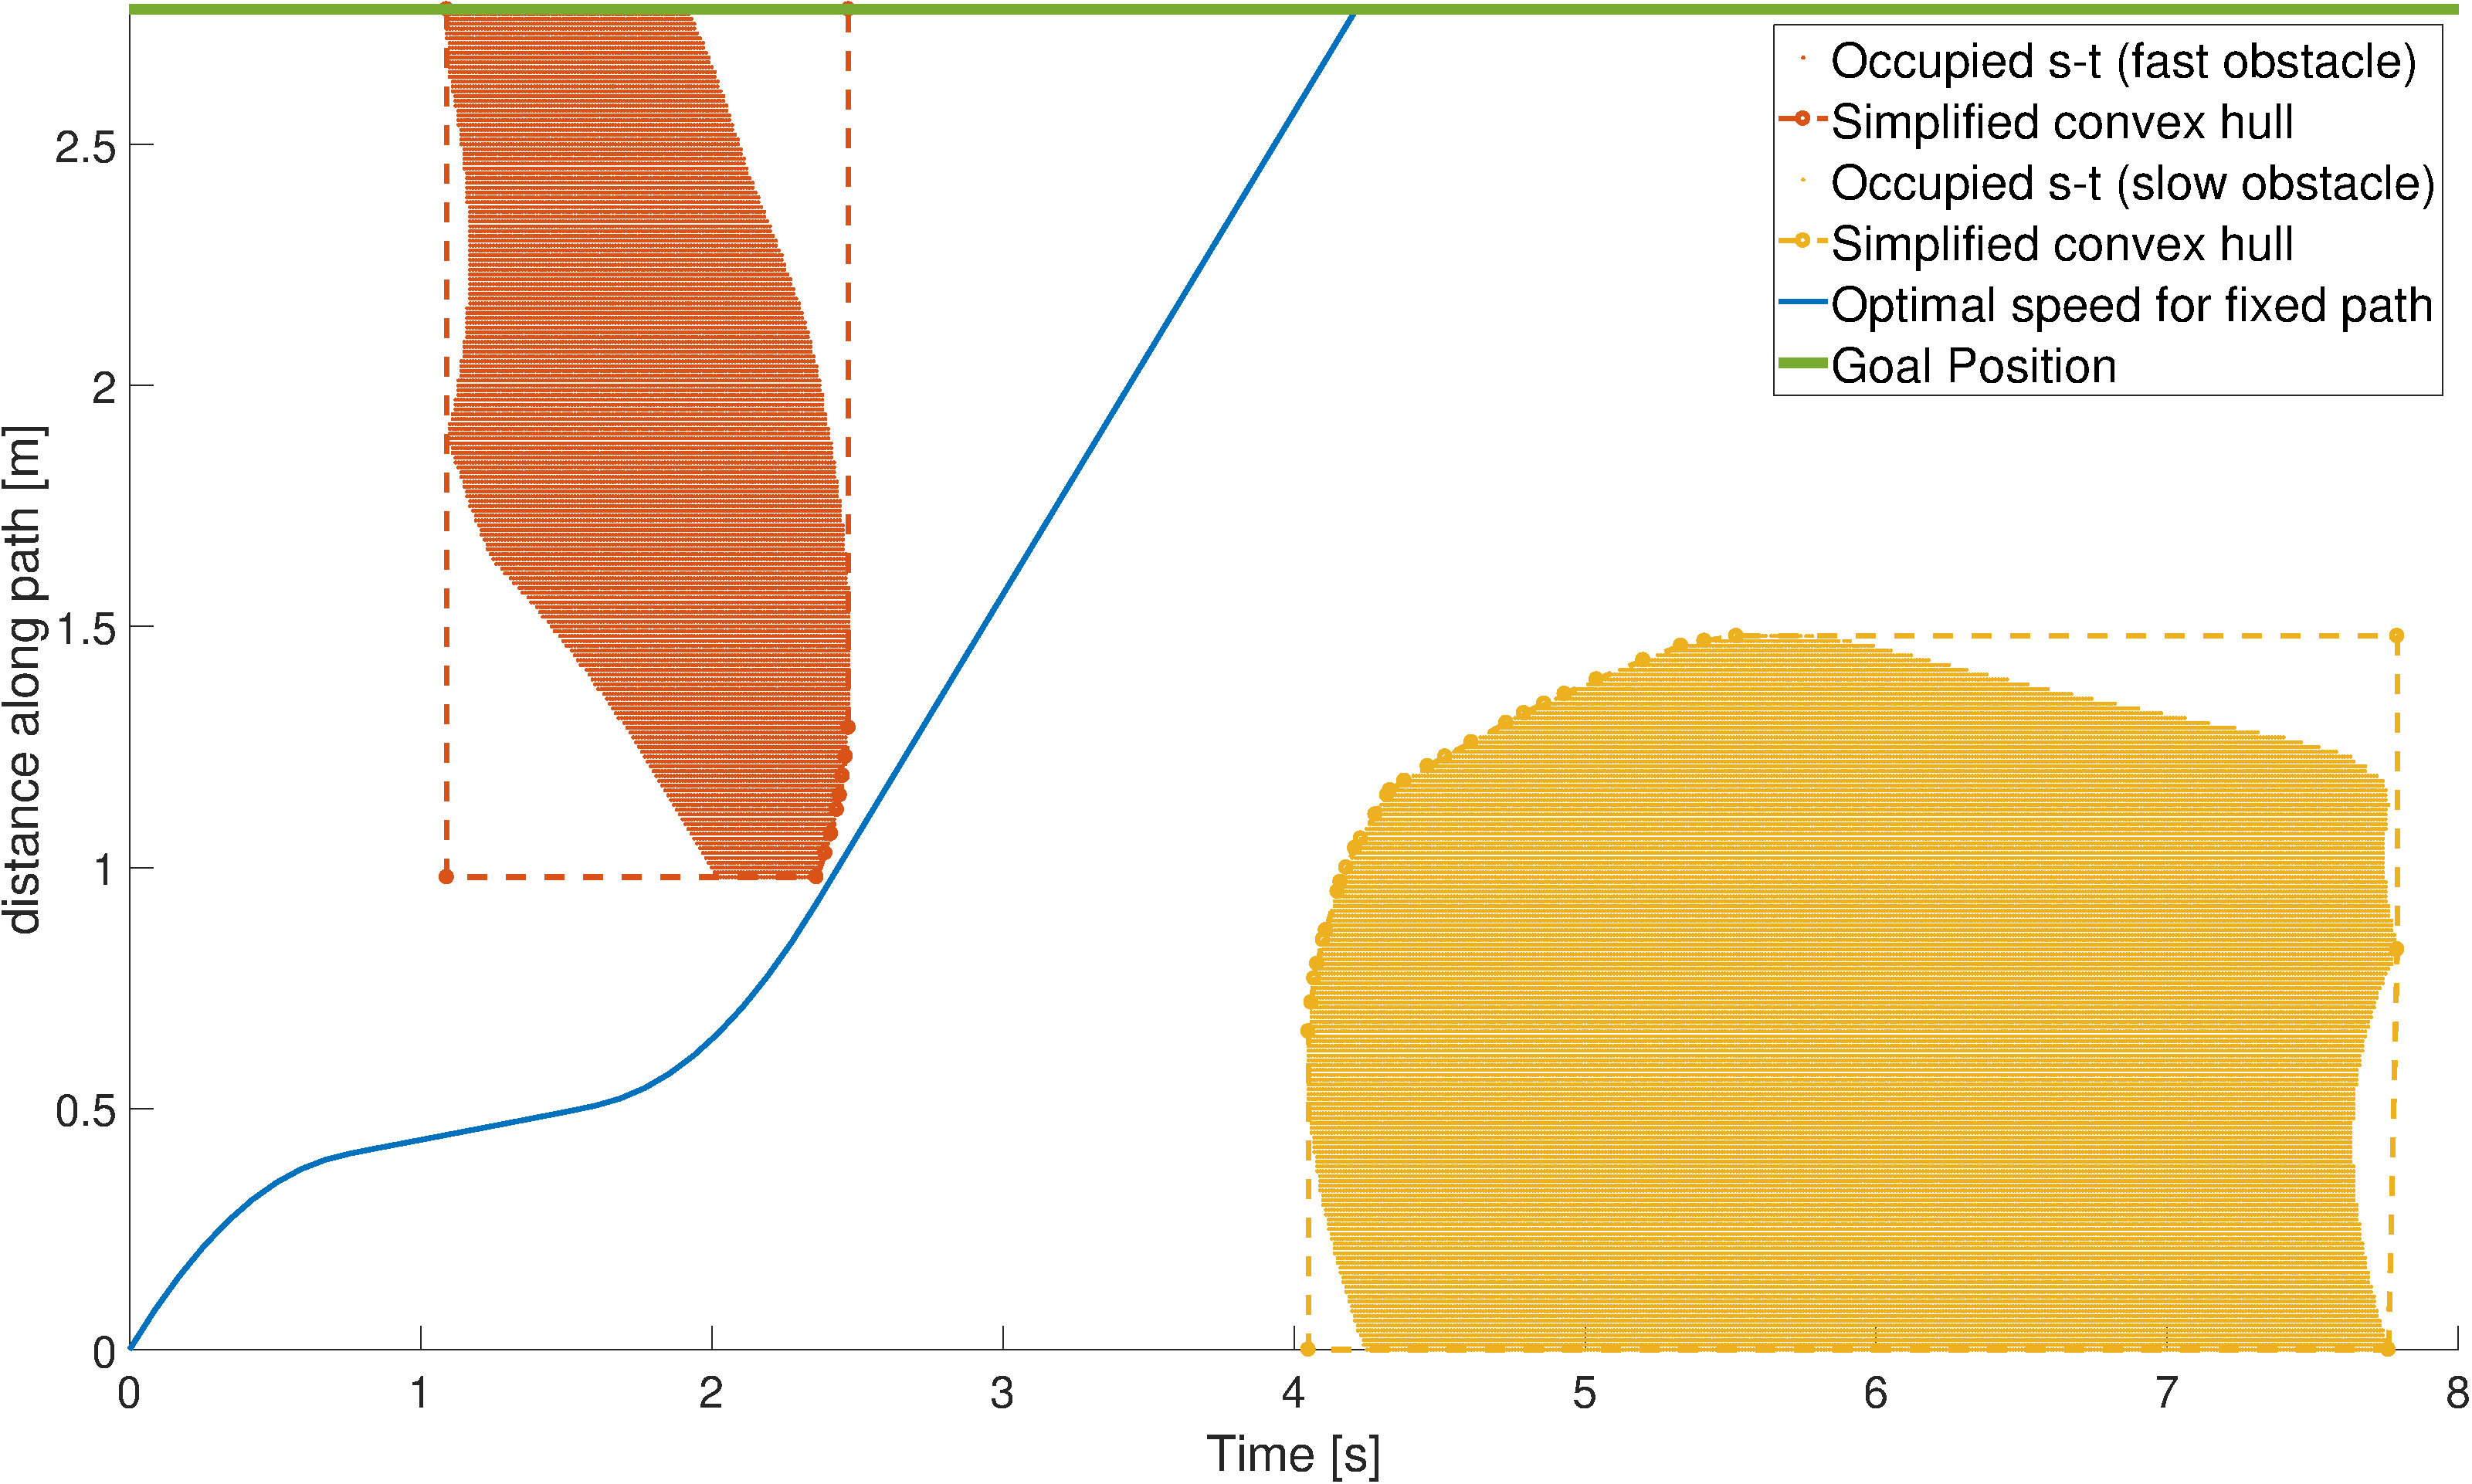
\includegraphics[width=\textwidth]{DVP_Solution.pdf}
\doublecaption{Dynamic motion planning among dynamic obstacles}{is achieved finding a path in the $s,t$-plane without intersecting the occupied cells. This results in an optimal speed profile for the sAMR, resulting in a collision-free motion.
\label{fig:DVP_Solution}}
\end{figure}


\newpage

\section{Socially Compliant Path Planning} \label{sec:HAPP}
The following section proposes solutions to different aspects reviewed in the literature study from \cref{sec:HARNrev} to obtain a path planner that will take into consideration several aspects of socially compliant navigation (\cref{sec:Comfort}).  An overview of the cooperation model developed by Trautman et al. \cite{TrautmanKrause2010,TrautmanEtAl2015} is given in \cref{sec:Cooperation} along with the most important mathematical models developed in their research. These additions have not been formally implemented in the source code presented in \cref{app:SourceCode}, but serve as guidelines in order to obtain a more socially compliant path planner.

\subsection{Enhancing comfort through social cost attribution} \label{sec:Comfort}
The impact on the comfort of humans with whom the driver and his wheelchair are interacting remains an important consideration even though the wheelchair is still guided by a person, as encoding those rules will make the planner inherently more socially acceptable. It is also possible that the driver has some disability making it more complicated for him to explicitly guide the wheelchair in a socially correct manner.

In order to obtain a path planner that inherently tries to follow social rules resulting in a more comfortable navigation as perceived by the surrounding people, a social cost should be computed for each path. After the intention of the driver has been calculated from the set of collision-free paths, weightings should be attributed to the path with the highest probability to be the user's intention and its associated social cost (a higher cost corresponds to a higher discomfort to the interacting person). The use of a cost function is preferred to the use of forbidden zones, since some situations require the wheelchair to enter someone’s intimate space in crowded spaces. 

A dynamic social cost map has been developed in \cite{ScandoloFraichard2011} starting from the guidelines of static personal space cost based on the study of proxemics \cite{Hall1966}. The authors have added other important factors, based on the back space of a person and his current motion direction. The use of back space puts an additional cost on moving right behind a person outside of his field of view. This additional cost during motion will adopt an elliptical form (rather than the circular form for static proxemics) and is proportional (and aligned) according to the velocity of the walking person.  This results in a dynamic personal space cost map displayed in \cref{fig:DynamicPersonalSpace}.

\begin{figure}[!htbp]
	\centering
    \includegraphics[width=0.5\textwidth]{DynamicPersonalSpace.jpg}
     \doublecaption{Dynamic personal space cost map.}{The blue area corresponds to the cost associated with the static proxemics. First, an infinite value is assigned to a distance resulting in a collision, followed by an exponential decrease depending on the different comfort zones (intimate, personal, social and public distance). The red area is the additional cost for being outside the field of view of the walking person. Finally, the yellow ellipse is the additional cost due to the motion of the person, reflecting the need to have a safe distance to stop (from \cite{ScandoloFraichard2011}).\label{fig:DynamicPersonalSpace}}
\end{figure}
 \vspace{-0.5em}
\subsection{Human-Robot Cooperation for Navigation in Crowed Spaces} \label{sec:Cooperation}
The research of Trautman et al. \cite{TrautmanKrause2010,TrautmanEtAl2015}, reviewed in \cref{sec:HRCrev}, has demonstrated that an independent motion planner will eventually fail even with perfect motion prediction of the agents surrounding the robot (recall \cref{fig:HuRoCo}). Eventually, when the density of a crowd of people exceeds a certain threshold, the planner will find no feasible paths and stop the robot or make it perform unnecessary evasive maneuvres. This is commonly called the FRP. Their solution to the FRP resides in the fact that people will adapt their own trajectories in order to make room for the wheelchair, thereby making it possible for everyone to reach their destination.

\begin{equation}
p_{\text{IGP}}({\bm f}^{(R)}, {\bm f^{(1:n)}}\vert {\bm z}_{1:t})=\frac{1}{Z}\psi({\bm f}^{(R)}, {\bm f^{(1:n)}})\prod\limits_{i=R}^{n}p({\bm f}^{(i)}\vert{\bm z}_{1:t}) \label{eq:IGPmodel}
\end{equation}

The developed prediction model, named Interacting Gaussian Process, is constructed by the interaction of the robot (${\bm f}^{(R)}$) and the other surrounding agents (${\bm f}^{(1:n)}$) with their corresponding observation (${\bm z}^{(1:n)}_{1:t}$), as displayed in \cref{eq:IGPmodel}. The probability over the whole trajectory from timesteps $1$ to $T$ (${\bm f}^{(i)} = f_{1}^{(i)}, \ldots, f_{T}^{({i})}$, $f^{(i)}_t = [x(t),y(t)]$) is modelled as a Gaussian Process. This Gaussian Process is defined by a mean function ($m^{(i)}$) and a kernel (covariance) function ($k^{(i)}$). The kernel function, which will model the shape of the agent's trajectories, is composed of a linear (nominal movement), Matern (mild curving) and noise (sensor noise) kernel. The different hyperparameters needed to define those terms are calculated based on training data (see \cite{TrautmanEtAl2015} for more information). The key function capturing the interaction between the agents is found in the interaction potential $\psi$ (see \cref{eq:InterPotFunc}), which requires only 2 tuning parameters: $h$ (controlling the ``safety margin'') and $\alpha$ (the strength of repulsion). $\vert f_{\tau}^{(i)}-f_{\tau}^{(j)}\vert$ is the Euclidean distance between agent $i$ and $j$ at time instance $\tau$. The interaction potential models the joint collision avoidance people adopt in crowded environments by lowering the provability a certain trajectory between two agents becomes from the moment they are too close to each other, since this would result in a possible collision between those two agents. $h$ and  $\alpha$ should be chosen in such a way that the minimal distance between two agents (observed from a training set) is enforced.

\begin{figure}[!tbp]
	\centering
    \includegraphics[width=0.5\textwidth]{InteractionPotentialFunction.pdf}
     \doublecaption{Influence of the two defining parameters for interaction potential between agent $i$ and $j$ at time instant $\tau$}{defined by \cref{eq:InterPotFunc}. ($\alpha$ and $h$) and is dependent on the (instantaneous) Euclidean distance between the two agents. This function lowers the probability that agent $i$ and $j$ are too close to each other at a given time instance $\tau$, reflecting the joint collision avoidance nature of humans. The distance is specified in pixels as an overhead camera was used during the experiments (adapted from \cite{TrautmanKrause2010}).\label{fig:InteractionPotentialFunction}}
\vspace{-1.5em}
\end{figure}

\begin{equation}
\psi({\bm f}^{(R)}, {\bm f^{(1:n)}})= \prod^{n}_{i=R}\prod^{n}_{j=i+1}\prod^{T}_{\tau=t}\left(1-\alpha\exp (-\frac{1}{2h^{2}}\vert f_{\tau}^{(i)}-f_{\tau}^{(j)}\vert)\right) \label{eq:InterPotFunc}
\end{equation}

From the derived model, one can design a LPPA that anticipates cooperation from the surrounding agents. However, ultimately, the observation ${\bm z}^{(1:n)}_{1:t}$ will still take priority, in case of non-cooperation. The path planning action is obtained by finding the maximum a posteriori from \cref{eq:IGPmodel} and by taking $f_{t+1}^{(R)\,\ast}$ as next waypoint for the navigation module, until the robot has arrived at its destination, shown in \cref{eq:NavMAP}.

\begin{equation}
({\bm f}^{(R)}, {\bm f^{(1:n)}})^{\ast}=\arg\max_{{\bm f}^{(R)},{\bm f^{(1:n)}}} P_{\text{IGP}} ({\bm f}^{(R)}, {\bm f^{(1:n)}}\vert {\bm z}_{1:t}) \label{eq:NavMAP}
\end{equation}

\section{Conclusion} \label{sec:DesignConclusion}
The developed clothoidal LPT uses a less restrictive curve geometry compared to the circular LPT used in \cite{DemeesterEtAl2012}, therefore providing a larger set of feasible paths. In situations where the sAMR has to travel through narrow openings, the clothoidal LPT will have a higher probability to find feasible paths, therefore providing better navigation assistance to the user of the wheelchair. The calculated paths connect the origin with discrete end poses in the surroundings of the robot, whilst taking into account the robot's constraints. 

Two alternatives have been compared to build the curve geometry, the Bézier curve and the clothoid. The latter has been selected for mainly two reasons: (i) it has a less restrictive formulation compared to the circle, since the curvature can vary linearly w.r.t. the path length; (ii) when driving at constant speed, the rotation speed of the wheels will only have to change linearly, making the clothoid easier to follow compared to the Bézier curve. To provide an even wider set of feasible paths, some paths consist of two clothoids. 

By using a predefined set of paths, the space the wheelchair will take along each path is known in advance and can be stored in a precomputed lookup table. The structure of the lookup table is optimized by containing for each occupied grid cell of the LPT the different paths occupying that certain grid cell and all the respective path lengths (when occupying that particular grid). In the online phase, the LPPA only has to compare the occupied cells from the grid-map containing all the obstacles of the environment with the lookup table. Each occupied cell will influence the total length of each path if the path length is shortened. It is important to note that the shape of both the robot and the obstacle can be arbitrary (convex or concave), but have to be converted in a grid-map.

A conceptual solution has been put forward for the calculation of the velocity profile when taking a path. The solution is based on the construction of an efficient search space in the distance-time collision space, relying on the fixed nature of the LPT and a given motion model of an obstacle to find a collision-free motion, compliant with the kinematic and dynamic constraints of the wheelchair. This efficient search-space has another interesting feature, notably the relative similarity of the collision-space occupied cells for similar paths, enabling grid search methods with a re-planning ability (e.g. D* or Incremental Phi*) to find quickly a solution for similar paths. 

Socially compliant path planning can take the shape of social costs resulting from the interaction of the user and his wheelchair with other individuals or crowds which can be attributed to selected paths. Whilst this additional social costing has not been formally implemented in the local path planning design as developed under \Cref{app:SourceCode}, such methodology remains compatible with the design of the clothoidal LPT. The human-robot cooperation model demonstrates promising results since it tackles one of the most important aspects in human navigation, the joint collision avoidance people engage in when walking in dense crowds. Without considering human behavior, the autonomous assisted navigation will not function properly in crowded environments.

By expanding the set of feasible paths of the LPT it is crucial to quantify the extra time needed when performing the online collision checking algorithm.  An in-depth evaluation of the clothoidal LPT will be discussed in \cref{cha:Eval}, by comparing it to the circular LPT.
\chapter{Evaluation of the Developed Local Path Planner} \label{cha:Eval}

\section{Introduction}
This section will evaluate the performances of the clothoidal LPT (the main focus of \cref{cha:Design} and contribution of this thesis) by comparing it with its predecessor, the circular LPT (discussed in \cref{sec:ColFreeTraj,sec:LPTreview}). First, the planning performance of both LPTs is assessed in \cref{sec:EvalPPP}. Two different path planning scenarios will be presented, requiring the planner to plan a trajectory through a narrow opening. One of the concerns raised in the conclusion of the design of the clothoidal LPT is the calculation time needed to calculate a path set that contains more paths compared to the circular path set. Time performances of both LPTs will therefore be analyzed in \cref{sec:EvalTP} in order to calculate the extra time needed to evaluate the additional paths from the clothoidal LPT. Some concluding remarks on the evaluation of the developed clothoidal LPT are given in \cref{sec:EvalConc}.

In order to objectively compare both LPTs, the curvature constraints on the path discussed in \cref{sec:WheelchairPlatform} are applied to the circular LPT. The procedure reviewed in \cref{sec:LPTreview} is performed, starting from 500 discrete input velocity pairs ($v,\omega$) but paths yielding a curvature $\kappa > \kappa_{max}$ are discarded. This results in a circular LPT composed of 250 trajectories (both forward and backward), shown in \cref{fig:MPCircVWPair_Eval}. The clothoidal LPT used for this evaluation is the same as shown in \cref{fig:LSLClothoid} and is composed of 1500 trajectories (forward and backward). Turning on the spot rotations were also discarded during this evaluation. 

\begin{figure}[!htbp]
	\centering
	\includegraphics[width=\textwidth]{MPCircVWPair_Eval.pdf}
	\doublecaption{Input velocities (left) integrated over a period of  $\Delta t = 4 s$ to obtain 250 circular paths complying with the kinematic constraints (right)}{(adapted from \cite{DemeesterEtAl2012}).
	\label{fig:MPCircVWPair_Eval}}
\end{figure}

\newpage

\section{Path Planning Performances} \label{sec:EvalPPP}
This section evaluates the path planning performance of the circular and clothoidal LPTs. The first benchmark consists of driving forward through a doorway (\cref{sec:EvalForwardDoor}); for the second benchmark, the wheelchair has to drive backwards into an elevator (\cref{sec:EvalBackElev}). Both benchmarks are inspired by real-world environments. The first consists of driving in the robot laboratory of the Department of Mechanical Engineering of the KU Leuven whilst the second involves entering the elevator in the corridor leading to this same laboratory.

\subsection{Forward Driving Through a Doorway} \label{sec:EvalForwardDoor}
In this situation, the sAMR has to drive through a doorway to enter the robot laboratory. First, a single successful situation is shown for both LPTs. Then, a thorough analysis between the circular and clothoidal LPT is provided, by trying to plan a path through the doorway by starting from different start poses in the corridor leading to the laboratory. An overview of the different planning performance outcomes along with a histogram are provided to evaluate both LPTs.

\subsubsection{Visual Inspection}
\Cref{fig:EnterRobotLab_Footprint} shows a successful, collision-free path going through the doorway using both LPTs. One can visually inspect the collision-free nature of each path by plotting the geometry of the wheelchair along the path and checking whether this collides with an obstacle. The green path indicates the path which is simulated to be the closest to the user's intention.

\begin{figure}[!htbp]
	\centering
    \includegraphics[width=0.45\textwidth]{EnterRobotLabCirc_Footprint.pdf}
    \hfill
    \includegraphics[width=0.45\textwidth]{EnterRobotLabCloth_Footprint.pdf}
     \doublecaption{Visual inspection of the selected path going through the doorway of the robot laboratory}{by plotting the footprint of the wheelchair along the selected path. (left) A successful path based on the circular LPT. (right) A successful path based on the clothoidal LPT. The footprint of the robot does not overlap with the environment, yielding collision-free paths for both LPTs.\label{fig:EnterRobotLab_Footprint}}
\end{figure}

\newpage

\subsubsection{Comparison Between the Circular and Clothoidal LPT}
%TODO not clear target and region
% Let's discuss this this evening
A uniform set of start poses are generated to assess the planning performances of both LPTs.
This is shown in \cref{fig:BenchmarkSetup} by performing the following steps:
\vspace{1em}
\begin{enumerate}
\item The test region (red polygon) defines uniformly spaced start positions (dots) with distance $dx$.
\item At each start position, a uniformly distributed set of start orientations, defined by $\theta_{range}$ and $\theta_{res}$ are aligned  with the target position (green star), creating a set of start poses. Then, each start orientation is rounded to the nearest multiple of $\theta_{res}$.
\item Poses resulting in a collision with the environment are removed.
\item If a path of the LPT originating from a start pose reaches the goal region (green polygon), that pose is defined as successful. The number of paths going through the goal region is not taken into account (e.g. \Cref{fig:EnterRobotLab_Footprint} shows a successful start pose for each LPT).
\item Successful start poses are divided in three cases:
\begin{enumerate}
	\item Only the circular LPT achieved to plan a path reaching the goal area
	\item Both LPTs achieved to plan a path reaching the goal area. 
	\item Only the clothoidal LPT achieved to plan a path reaching the goal area.
\end{enumerate}
\end{enumerate}

\begin{figure}[!htbp]
	\centering
	\includegraphics[width=.8\textwidth]{BenchmarkSetup.pdf}
    \doublecaption{Setup parameters of the uniformly distributed set of start poses.}{Start positions are uniformly spread with a distance of $dx=10cm$ between each other. The discrete set of start orientations are defined by $\theta_{range}= 90\degree$ and $\theta_{res}=\frac{90}{32}\degree$ and are aligned with the goal target. The last operation consists of rounding the start orientations to the nearest multiple of $\theta_{res}$ value to ensure a better uniformity.\label{fig:BenchmarkSetup}}
\end{figure}

\vspace{1em}

The final outcome when following this procedure is shown in \cref{fig:EnterRobotLabEval_result} along with a histogram of the occurrence of the three different cases in \cref{fig:EnterRobotLabEval_hist}. The unique successful start poses based on circular, common and clothoidal LPTs are shown respectively in red, black and green. The width of the doorway from the corridor to the robot laboratory is 80 cm while the width of the wheelchair is 60cm.

\newpage

From this outcome, several important conclusions can be drawn:
\begin{itemize}
\item Since straight paths are common to both LPTs, poses in front of the goal region obtain the same result for the circular and clothoidal LPT.
\item The majority of the paths from start poses at the lower end of the figure are achieved by the circular LPT. This is because those paths only require a circular arc to enter the doorway. Since the circular LPT is composed of a uniformly spread set of circular trajectories, this LPT is favored, compared to the clothoidal LPT.
\item From the moment the required trajectory is more complex (for example, \cref{fig:EnterRobotLab_Footprint} (right) the clothoidal LPT is the only LPT able to plan a path.
\item As per the histogram provided in \cref{fig:EnterRobotLabEval_hist}, the majority (87\%) of the poses with a successful path are generated by the clothoidal LPT, which demonstrates that for this first benchmark, the lack of uniformly spread circular trajectories is not so crucial, as only 13\% of the total amount of successful start poses are uniquely found by using the circular LPT.
\end{itemize}

\begin{figure}[!htbp]
	\centering
    \includegraphics[width=0.85\textwidth]{EnterRobotLabEval_result.pdf}
     \doublecaption{Successful start poses for each LPT finding a path through the doorway of the robot laboratory}{separated in the three different cases.\label{fig:EnterRobotLabEval_result}}
\end{figure}

\begin{figure}[!htbp]
	\centering
    \includegraphics[width=0.5\textwidth]{EnterRobotLabEval_hist.pdf}
     \doublecaption{Histogram showing the outcome of the different cases of driving through the doorway of the robot laboratory.}{There are in total 3604 successful start poses, from which 1708 are common to both LPTs. Whereas 460 are only from the circular LPT and 1436 from the clothoidal LPT. \label{fig:EnterRobotLabEval_hist}}
\end{figure}

\newpage

\subsection{Backwards Driving in an Elevator} \label{sec:EvalBackElev}
In this situation, the sAMR must drive in reverse from a corridor into an elevator. First, a single successful situation is shown for both LPTs. Then, an in-depth comparison between the circular and clothoidal LPTs will be given of their attempts to reach the elevator by starting from different start poses in the corridor leading to the elevator. An overview of the different planning performances along with a histogram will be provided to evaluate both LPTs. This benchmark is inspired by the situation described in \cite{VanderPoortenEtAl2012}, where the circular LPT is unable to plan a trajectory leading to the elevator when the wheelchair is located in the corridor. The width of the elevator is 90 cm while the width of the wheelchair is 60cm.

\subsubsection{Visual Inspection}
\Cref{fig:EnterLift_Footprint} shows a successful, collision-free path going in reverse through the doorway of the elevator whilst using both LPTs. One can visually inspect the collision-free nature of each path by plotting the geometry of the wheelchair along the path and checking whether this collides with an obstacle. The green path indicates the path simulated to be the closed to the user’s intention.

\begin{figure}[!htbp]
	\centering
    \includegraphics[width=0.45\textwidth]{EnterLiftCirc_Footprint.pdf}
    \hfill
	 \includegraphics[width=0.45\textwidth]{EnterLiftCloth_Footprint.pdf}
     \doublecaption{Visual inspection of the selected path going in reverse through the doorway of the elevator}{by plotting the footprint of the wheelchair over the selected path. (left) A successful path based on the circular LPT. (right) A successful path based on the clothoidal LPT. The footprint of the robot does not overlap with the environment, proving that both cases yield a collision-free path.\label{fig:EnterLift_Footprint}}
\end{figure}

\newpage

\subsubsection{Comparison Between the Circular and Clothoidal LPT}
The same procedure as provided in \cref{fig:BenchmarkSetup} is applied for this benchmark.  From this outcome, several important conclusions can be drawn:
\begin{itemize}
\item The majority of the common start poses are found at the right of the start region, before the beginning of the corridor. 
\item From the moment the start pose of the wheelchair is located further away in the corridor, only the clothodial LPT manages to find a trajectory to the elevator.
\item This outcome confirms the comment in \cite{VanderPoortenEtAl2012}, that from the moment a trajectory leading to a certain destination becomes too complex, the circular LPT is unable to find a path. Recall from \cref{sec:PlanRec} that the collision-free trajectories also model the user’s intention. Since no paths can be found in the corridor leading to the elevator, there will be only limited guidance for the wheelchair user. By contrast, the clothoidal LPT performs very well in the corridor and is able to plan a path to the elevator from far in corridor.
\item The above outcomes are confirmed by the histogram shown in \cref{fig:EnterLiftEva_hist}. Nearly all the start poses are successful when using the clothoidal LPT (98\%).
\end{itemize}

\begin{figure}[!htbp]
	\centering
    \includegraphics[width=\textwidth]{EnterLiftEval_result.pdf}
     \doublecaption{Successful start poses for each LPT planning a path backwards into an elevator}{separated in the three different cases\label{fig:EnterLiftEval_result}}
\end{figure}

\begin{figure}[!htbp]
	\centering
    \includegraphics[width=0.5\textwidth]{EnterLiftEva_hist.pdf}
     \doublecaption{Histogram illustrating the outcome of the different cases for planning a path backwards into an elevator.}{There are in total 2904 successful start poses, from which 1224 are common to both LPTs. Whereas 64 are only from the circular LPT and 1616 from the clothoidal LPT. \label{fig:EnterLiftEva_hist}}
\end{figure}

\newpage

\section{Time Performances} \label{sec:EvalTP}
One important consequence of augmenting the number of paths in the set of feasible trajectories of the LPTs is the time needed to adjust the path length. Since the clothoidal LPT has six times more paths than the circular LPT and assuming a stable computing capacity, applying the clothoidal LPT would be impracticable if the increase in time required would be fully proportional to the increased number of paths. 

This section will investigate two different cases. First, in \cref{sec:EvalTimeSingle} a single occupied cell of the lookup table presented in \cref{sec:OBLT} will be simulated as occupied. Then, in a more realistic scenario, the sAMR is positioned in several poses in the environment as shown in \cref{fig:EnterLiftEval_result}, resulting in a different amount of occupied cells from the lookup table \cref{sec:EvalTimeMulti}.

The presented benchmarks were run on a computer with an Intel\textregistered~Core\texttrademark~i5-4460 quad core 3.20GHz CPU with 16GB of memory. Benchmark scripts were written in MATLAB. A better time performance is therefore expected when this developed LPPA would be implemented in a more efficient programming language (e.g. C/C++), as the results available for the circular LPT \cite{DemeesterEtAl2012}. The relative comparison between the two LPTs remains however relevant.

\subsection{Single Occupied Cell} \label{sec:EvalTimeSingle}
This benchmark will show the time needed to adapt the path length of both LPTs when a single cell of the LPT is simulated to be occupied. This has been visually demonstrated in \cref{fig:LPT_LT}. To avoid any bias with respect to the row-index in the lookup table, an equally spread set of occupied cells will be picked from the whole lookup table. The algorithm used for this search is the build-in MATLAB function ``ismember'' which was applied on a hash-table form of the lookup table to further optimize speed. This hash-table form enables a scalar-search compared to a much slower row-search. This speed-up optimization was found in \cite{Altman2014} and has approximately accelerated the search time by a factor of 50.

\Cref{fig:TimeBench_SingleObs_mat} (left) shows a histogram of the obtained execution time of this benchmark applied to the circular and clothoidal LPT. The circular LPT proves to be more time efficient, which was expected, since this LPT contains six times less paths compared to the clothoidal LPT. The median execution time of the circular LPT is 0.265 ms compared to 0.608 ms for the clothoidal LPT (2.3 times slower). 


Another important relationship that can be analyzed with this benchmark is the execution time dependency of the affected paths (for 1 occupied cell). This is shown in \cref{fig:TimeBench_SingleObs_mat} (right), where each dot indicates a single experience. From this figure, a clear dependency on the number of paths can be seen, with the linearly increasing minimal execution time, for a cell affecting a particular amount of paths. This reflects the linear increasing time needed to adapt the length of each individual path. The vertical difference in time can be explained by a varying time needed for searching the cell in the lookup table.

%TODO  read this again
As expected, the maximum number of paths from the circular LPT (250) is to be found on the plot in red. This is not the case for the clothoidal LPT composed of 1500, however the cell containing the maximum amount of paths is 337. Since not every path from the clothoidal LPT starts at the origin due to the EP (recall \cref{sec:EP}, some trajectories are composed of 2 clothoids). There is a parent-child from clothoids originating from a certain EP, since they are automatically marked as fully blocked from the moment the path leading to that EP has been shortened. This structural relationship has therefore led to an increase in the speed for the collision checking, since otherwise the graph displayed in \cref{fig:TimeBench_SingleObs_mat} (right) would have continued linearly to 1500 paths affected by a single cell. 

\begin{figure}[!htbp]
	\centering
	\includegraphics[width=0.45\textwidth]{TimeBench_SingleObs_mat_hist.pdf}
    \hfill
	\includegraphics[width=0.45\textwidth]{TimeBench_SingleObs_mat_PathInfluence.pdf}
    \doublecaption{Execution time needed to adapt the path length of the circular and clothoidal LPT for a single obstacle.}{Occupied cells are equally spread over the whole lookup table to obtain cells affecting a different number of paths. (left) Histogram of the resulting execution time. The circular LPT with a median of 0.265 ms is 2.3 times faster as the clothoidal LPT with a median of 0.608 ms. (right) When plotting the executing time over the number of paths the cell affects, a clear linear relationship is visible for the minimal executing time for both LPTs, reflecting the linear increasing time needed to adapt each path. The varying amount of execution time for a given number of paths per cell can be explained by the difference in time needed to find that cell in the lookup table.\label{fig:TimeBench_SingleObs_mat}}
\end{figure}

\subsection{Multiple Occupied Cells} \label{sec:EvalTimeMulti}
This benchmark will evaluate the execution time of both LPTs in a simulated environment (\cref{fig:EnterLiftEval_result}). Different start poses are tested resulting in a varying amount of occupied cells from the environment matched with cells in the lookup table. \Cref{fig:TimeBench_MultiObs} (left) shows a histogram of the execution time needed to adapt each path from the LPTs. The relative difference in execution time is more visible in this case compared to a single occupied cell. For this benchmark, the median execution time of the circular LPT is 29 ms compared to 114 ms for the clothoidal LPT; the clothoidal LPT is therefore 3.9 times slower.

\Cref{fig:TimeBench_MultiObs} (right) shows the execution time of the trajectory adjustment over the number of occupied cells. No clear relationship can be observed, which indicates that the process of matching occupied grid cells from the environment with the precomputed cells in each LPT is the most expensive operation. One can note the slightly more grouped nature (already visible from the histogram) of the circular LPT compared to the clothoidal LPT.

\begin{figure}[!htbp]
	\centering
	\includegraphics[width=0.45\textwidth]{TimeBench_MultiObs_hist.pdf}
    \hfill
	\includegraphics[width=0.45\textwidth]{TimeBench_MultiObs_ObstacleInfluence.pdf}
    \doublecaption{Execution time needed to adapt the path length of the circular and clothoidal LPT for a simulated environment.}{Different poses are used to obtain a varying number of triggered cells when an obstacle in the surroundings of the sAMR matches one in the precomputed lookup table. (left) Histogram of the resulting execution time. The circular LPT with a median of 29 ms is 3.9 times faster as the clothoidal LPT with a median of 114 ms. (right) When plotting the executing time over the number of occupied cells from the lookup table, no clear relationship can be found. This indicates that the search function is the most time-consuming process.\label{fig:TimeBench_MultiObs}}
\end{figure}
\newpage

\section{Conclusion} \label{sec:EvalConc}
This chapter has evaluated two critical performance criteria of the developed local path planner designed in \cref{cha:Design}, the clothoidal LPT by comparing it to the circular LPT. The clothoidal LPT has a less restrictive formulation compared to the circular LPT, therefore enabling more complex curves. 

By having six times more paths compared to its predecessor, the clothoidal LPT achieves an improved path planning performance. This has been demonstrated in two different situations. The clothoidal is especially successful in situations that either require a complex path to achieve a possible destination due to the environment as per the first experiment, or that have an unfavorable start pose, as per the second experiment.

 A major concern is the extra time needed to adapt the paths from the clothoidal as against those of the circular LPT. The time performance of each LPT has been evaluated, in an experience whereby both LPTs were tested in an environment with varying test poses. This resulted in varying the number of occupied grid cells from the environment matching the cells from the lookup table. Results of this experience showed that the clothoidal LPT needed nearly four times more computing time to adjust each individual path length as compared to the circular LPT (median value of 114 ms compared to the 29 ms). 
 
 Although these experiments have been performed in MATLAB and implementing this in a more efficient programming language (e.g. C/C++) would minimize the impact of the increased computing time, it may be important to achieve further efficiency improvements. The main reason behind the large amount of paths for the clothoidal LPT is due to the use of EPs as explained in \cref{sec:EP}. These are uniformly spread over the local grid, resulting in a symmetric expansion of the paths of the LPT (recall \cref{fig:LSLClothoid}). Two possible improvements regarding the position of the EPs could be implemented:
\begin{enumerate}
\item An asymmetric location of the EPs is applied, yielding for example 6 different zones (straight, left, right for forwards or backwards motion). Six different LPT are then available for the LPP then only has to choose between the six possible LPTs, for instance straight-forward or left-backwards.
\item The choice of the EP positions is performed online and is not necessarily restricted to 2 successive clothoids.  The fast calculations of the LPT could therefore be combined with the flexibility of DMP by using a fast planner for several successive EPs. 
\end{enumerate}
Both solutions would achieve a more efficient clothoidal LPT, by taking the environment or the previous user’s intention into account, without interfering with the improved planning capacity resulting from the higher flexibility of the clothoid.

\chapter{Future Work} \label{cha:FutWork}
This chapter presents possible future work building on the outcome of the present thesis, or on particular aspects put forward in it with the aim to further improve the reliability of the LPP as reviewed in \cref{sec:ReqLPP}.

The implementation of human-aware navigation will lead to a navigation system that helps the user of the sAMR to adopt a more socially compliant motion. This can be done by using a social cost model attributing a higher cost to paths leading to asocial behavior. The human-robot cooperation model developed in \cite{TrautmanKrause2010,TrautmanEtAl2015} appears promising in this regard and once implemented may enable the wheelchair to navigate in an efficient and safe manner through densely crowded areas.

The computational efficiency of the clothoidal LPT is unfavorable compared to the circular LPT. This can be addressed by looking at ways to lower the number of paths to be calculated. The position of the EPs could be determined by the environment or by the user’s intention. This will lower the amount of paths in the LPT resulting in a faster execution time while still keeping the flexibility of the clothoidal paths. Two possible solutions were put forward in \cref{sec:EvalConc}, one using several fixed sets of asymmetrical LPTs and the other, by deciding online the location of $n$ successive EPs.

The motion control unit, needed to execute and follow a planned path has not been discussed in this thesis. This controller will cope with the influence on the castor wheels (\cref{sec:WheelchairPlatform}) which the planner has omitted. These castor wheels will have an influence on the first few centimetres of the executed path if they are not aligned correctly. This yields a controller with a much higher dimensional space compared to the current 3D planner ($x,y,\theta$) and will (at least) have to include the orientation of the different castor wheels.

Context-based navigation can be implemented by the use of semantic knowledge-based maps. These maps would contain information that could help during the navigation. For example, when a sAMR is driving in a train station and knows it is in the ticket office, it should not expect any cooperation from the person waiting in line. Therefore, context-aware navigation could also lead towards a more socially compliant navigation.

\newpage

Finally, the COP used to plan a motion with dynamic obstacles is a costly operation, which can only be performed for a small subset of the calculated paths. A better method could be based on a grid planner benefiting from the similarity between the distance-time collision space from similar paths, like the D* or Incremental Phi* planner.
\chapter{Conclusion} \label{cha:Concl}
This thesis has contributed to the ongoing research of the Department of Mechanical Engineering of the KU Leuven on Wheelchair Navigation Assistance. The goal of this work was to expand the current LPP, the circular LPT, with a more flexible curve, enabling it to plan more complex paths to a desired destination and therefore providing better navigation assistance, as the collision-free paths are used to model the user's intention along with the path the sAMR will execute.

The developed clothoidal LPT consists of a set of kinematically feasible trajectories based on clothoids (a curve whose curvature changes linearly with its arc length) starting from the current pose of the robot and connecting it with a set of discrete end-poses in the surrounding of the robot. With this fixed set of trajectories, a lookup table is built in order to efficiently obtain accurate collision-free paths by adapting the length of each trajectory.

Several simulations were designed to evaluate the improved planning performances of the clothoidal LPT as compared to its predecessor, the circular LPT. These experiments confirmed that by adopting a more flexible curve geometry, the clothoidal LPT’s ability to plan a passage through a narrow opening was less dependent on the current pose of the sAMR as its predecessor.  This has increased the amount of paths in the clothoidal LPT by six which has led in turn to an increase in overall executing time by four. The main improvement that could be made to the current design of the clothoidal LPT in terms of computing time would be to change the current locations of the EPs, which are the main reason behind the large increase of paths, and decide on their location more accurately.

The focus of the developed LPPA has been on curve geometry and path length adaptation for static obstacles. A conceptual solution using an efficient search space (the distance-time collision space) has been put forward to cover also for the prevention of collision in a dynamic environment. Building on the respective strengths of the LPT and optimal motion generation, this solution provides an optimal speed profile resulting in a collision-free motion for a fixed path in an environment with dynamic obstacles. This could be extended by using a grid search algorithm with re-planning abilities, since there is a similarity between the occupied space caused by the dynamic obstacles between similar paths, resulting in faster calculation time.

The need for a cooperative planner, which anticipates the cooperation of people in dense crowds has been presented as a possible solution to the FRP and would therefore enable the sAMR to navigate efficiently and safely in densely populated environments. Social compliant robotic navigation would be achieved by integrating a dynamic social cost map accounting for discomfort caused to interacting persons by the wheelchair as it moves through crowds.
\appendixpage*
\appendix
\chapter{Bézier Curve Calculations} \label{app:BezierCurve}
\vspace{-2em}
This appendix further elaborates the mathematical properties of the Bézier curve and provides an elaborated overview of the COP formulation to obtain a set of kinematically feasable trajectories for the sAMR given a set of CEPs.

\section{Mathematical Formulations and Derivatives} \label{sec:BezierMathGen}
The curvature ($\kappa$) of the Bézier curve needs to be calculated since this is present in the objective function and in the contrains of the COP \cref{eq:BezierCOP}. The first step is to transform the general formulation shown in \Cref{eq:BezierCurveGeneralApp} and rearange the terms in it's matrix formulation displayed in \Cref{eq:BezierCurveMat}. To calculate the derivative of the Bézier curve, another property is used:  the derivative of Bézier curve of order $n$, is another Bézier curve of order $n-1$ \cite{Sederberg2016}, see \cref{eq:BezierCurveGeneralDerivative}. The same method can be applied in order to calculate the second order derivative $\bm{B}''(n,u)$. The curvature is calculated as shown in \cref{eq:curvature}. The first and second derivative are shown in matrix form in \cref{eq:BezierCurveMatFirstDev,eq:BezierCurveMatSecondDev}.

\begin{equation} 
\bm{B}(n,u) = \sum_{i=0}^{n-1}
\underbrace{ \begin{pmatrix} n-1 \\ i \end{pmatrix}}_\text{binomial term} \cdot~
\underbrace{(1-u)^{n-1-i} \cdot u^i}_\text{polynomial term}
\cdot~\underbrace{ P_i}_\text{control point}
\label{eq:BezierCurveGeneralApp}
\end{equation}

\begin{equation}
B(u) =
\begin{bmatrix}
u^3 & u^2 & u & 1  
\end{bmatrix}
\begin{bmatrix*}[r]
-1 &  3 & -3 & 1\\ 
 3 & -6 &  3 & 0\\ 
-3 &  3 &  0 & 0\\ 
 1 &  0 &  0 & 0 
\end{bmatrix*}
\begin{bmatrix}
P_1  \\ P_2 \\ P_3 \\ P_4 
\end{bmatrix} \label{eq:BezierCurveMat}
\end{equation}

%TODO
% CHECK AGAIN
\begin{equation} \label{eq:BezierCurveGeneralDerivative}
\bm{B}'(n,u) = \sum_{i=0}^{n-2}
\begin{pmatrix} n-1 \\ i \end{pmatrix} \cdot~
(1-u)^{n-1-i} \cdot u^i
\cdot~( P_{i+1}-P_{i})
\end{equation}


\begin{align}
B'(u)  &=
\begin{bmatrix}
u^2 & u & 1  
\end{bmatrix}
\begin{bmatrix*}[r]
 1 & -2 & 1\\ 
-2 &  2 & 0\\ 
 1 &  0 & 0 
\end{bmatrix*}
\begin{bmatrix}
P_1-P_2  \\ P_2- P_3  \\ P_3- P_4 
\end{bmatrix} \label{eq:BezierCurveMatFirstDev}\\
B''(u) & =
\begin{bmatrix}
u & 1  
\end{bmatrix}
\begin{bmatrix*}[r]
 1 & -2\\ 
-2 &  2
\end{bmatrix*}
\begin{bmatrix}
P_1- 2 P_2 + P_3  \\ P_2 - 2 P_3 + P_4 
\end{bmatrix}&  \label{eq:BezierCurveMatSecondDev}
\end{align}

\section{Constrained Optimization Problem Formulation}
The problem of connecting one pose to another is mathematically described as a two point G1 Hermite interpolation. When using a cubic Bézier curve, two degrees of freedom are left when connecting one arbitrary pose $\bm{p_s}=[x_s, y_s, \theta_s]$ to another $\bm{p_e}=[x_e, y_e, \theta_e]$. A COP is formulated satisfying the kinematic contraints while minimizing bending energy of the curve, resulting in a more comfortable path for the drive. The resulting COP yields a non-convex problem which is subjected to local minima, a optimal solution is therefore hard to find. The calculation of the COP is done with Casadi, developed at the Optimization in Engineering Center of the KU Leuven \cite{Andersson2013}. 

\begin{mini!}
{P_{1:4}}{ f(P_{1:4}) = \int_0^1{\kappa(u)^2du }
\label{eq:ObjectiveFunctionApp}}
{\label{eq:BezierCOP}}
{}
\addConstraint{P_1-P_s}{=[0,0]} \label{eq:startPos}
\addConstraint{ \begin{bmatrix}-\tan\theta_s & 1\end{bmatrix}(P_2 - P_s)^T}{=0} \label{eq:startOrient}
\addConstraint{P_4-P_e}{= [0,0]} \label{eq:endPos}
\addConstraint{ \begin{bmatrix}-\tan\theta_e & 1\end{bmatrix}(P_e - P_3)^T}{=0} \label{eq:endOrient}
\addConstraint{\kappa(u)^2- \kappa_{max}^2}{\leqslant 0} \label{eq:maxCurvature}
\addConstraint{lb_x\leqslant}{\ P_{x,2-3}}{\leqslant ub_x} \label{eq:boundX}
\addConstraint{lb_y\leqslant}{\ P_{y,2-3}}{\leqslant ub_y.} \label{eq:boundY}
\end{mini!}
\begin{flalign}
	\text{With:}& \nonumber \\
	& P_{1:4}, \ \text{the four control point defining the cubic Bézier curve} \nonumber \\
	& u =0:\Delta u:1, \ \text{parameter to construct the curve} \nonumber \\
	& \kappa(u) = \frac{B'(u) \times B''(u)}{\|B'(u)\|^3} = \frac{x'y''-y'x''}{(x'^2+y'^2)^{\nf{3}{2}}}, \ \text{curvature} \label{eq:curvature} \\
	& \kappa_{max}, \ \text{maximum allowed curvature} \nonumber \\
	& P_{s,e}, \ \text{start and end position} \nonumber \\
	& lb_{x,y}, \ \text{lower bound on the x,y-position of the control points} \nonumber \\
	& ub_{x,y}, \ \text{upper bound on the x,y-position of the control points} \nonumber &
\end{flalign}
\chapter{Source Code}\label{app:SourceCode}
The source code developed for this thesis is available at the following GitLab repository \cite{Denis2017} (\url{https://gitlab.mech.kuleuven.be/rob-mastertheses/kdenis-2016}) and can be found in the src directory. The most important notes are available in the README in this directory. More information is given in each function if needed. The same information has been uploaded as ``Digital Appendix'', also under the src folder. 

\section{Directory Organization}
\begin{itemize}
\tightlist
\item ROOT: contains all the most important scripts and functions.
\item data\_img: contains all the used maps and robot's footprint / geometry.
\item data\_mat: contains all the precomputed data (paths and corresponding lookup tables) for fast use of the local path planner in  the ``main'' example. Also for the plot scripts.
\item helper\_external:  contains all the files which are \emph{NOT} written by Kevin DENIS, but found on the web (mostly MATLAB file exchange or stackoverflow).
\item helper\_func: contains all the sub-functions needed for the main functions from the root.
\item helper\_plot: contains all functions needed for plotting scripts.
\item scripts\_plot: contains all the scripts which were used to create  figures.
\end{itemize}

\backmatter
% The bibliography comes after the appendices.
% You can replace the standard "abbrv" bibliography style by another one.
\bibliographystyle{abbrv}
\bibliography{references}
\end{document}